% The values have been rounded to the nearest 2,000 in this plot., 12,000 Figure 1.20 29 Page

\chapter{데이터 소개}
\label{introductionToData}

%\begin{tipBox}{\tipBoxTitle[Chapter Goal:]{Thinking about data}
%Understand basics about data organization, data types, numerical summaries of data, graphical summaries of data, and foundational techniques for data collection. We begin and end the chapter with case studies.}
%\end{tipBox}


과학자들은 엄격한 방법과 주의깊은 관찰을 통해서 질문에 답을 탐구한다.
이러한 관찰 -- 연구수첩, 설문조사, 실험을 통해 수집 -- 결과가 통계 조사에서 중추적인 역할 구성하고 \term{데이터(data)}라고 부른다. 통계는 자료를 수집하고, 분석하고, 데이터로부터 결론을 도출하는 최상의 방법을 연구하는 학문이다.
일반적인 조사 과정 맥락에서 통계를 두는 것이 도움이 된다:

\begin{enumerate}
\setlength{\itemsep}{0mm}
\item 질문 혹은 문제를 식별한다.
\item 주제와 관련된 데이터를 수집한다.
\item 데이터를 분석한다.
\item 결론을 구성한다.
%\item Make decisions based on the conclusion.
\end{enumerate}

학문으로 통계는 2-4개 단계를 객관적이고, 엄격하며, 효율적으로 만드는데 집중한다. 즉, 통계는 주요 구성요소가 세가지다: 데이터를 얼마나 잘 수집하는가? 데이터를 어떻게 분석하는가? 그리고, 분석으로부터 무엇을 추론할 것인가?

과학자가 조사하는 주제는 과학자가 끝임없이 질문하는 질문만큼 다양하다.
하지만, 이러한 조사의 상당부분은 일부 자료수집기법, 분석 도구, 통계적 추론의 근본개념으로 해결될 수 있다.
이번 장에서 간략히 들여다보고 다른 주제는 이책 나머지 부분에서 다뤄질 예정이다.
각각에 대한 기본 원칙을 소개하고 기본 도구 일부를 학습해 나갈 것이다.
다른 분야 응용사례를 마주할 것인데, 일부는 과학과 꼭 연관되어 있지는 않지만, 그럼에도 불구하고, 통계조사를 통해 혜택을 받을 수 있다.

\section[Case study: using stents to prevent strokes]{사례 연구: 뇌졸중을 방지에 사용되는 스텐트(Stent)\sectionvideohref{youtube-nEHFF1ADpWE&list=PLkIselvEzpM6pZ76FD3NoCvvgkj_p-dE8}}
\label{basicExampleOfStentsAndStrokes}

\index{데이터(data)!뇌졸증|(}

~\ref{basicExampleOfStentsAndStrokes} 절에 통계학의 전통적 도전과제가 소개되어 있다: 치료효능 평가. 이번 절에서 사용되는 용어는 본 교과서 후반부에서는 모두 수정될 것이다. 현시점에서 계획은 통계가 실무에서 수행하는 역할에 대해 느낌만 잡기 바란다.

이번 절에서는 뇌졸증 위험 환자를 치료하는데 사용되는 스텐트의 유효성을 연구하는 실험을 고려한다.\footnote{Chimowitz MI, Lynn MJ, Derdeyn CP, et al. 2011. Stenting versus Aggressive Medical Therapy for Intracranial Arterial Stenosis. New England Journal of Medicine 365:993-1003. \urlwofont{http://www.nejm.org/doi/full/10.1056/NEJMoa1105335}. 본 조사연구를 보도하는 NY 타임즈 기사: \urlwofont{http://www.nytimes.com/2011/09/08/health/research/08stent.html}.} 
스텐트(stent)는 혈관내부에 장착하는 장치로 심장 쇼크 이후 환자회복을 돕고, 추가적인 심장마비 혹은 경색 위험을 줄여준다.
많은 의사들이 뇌졸증 위험이 있는 환자에게도 비슷한 효능이 있을 것이라는 희망을 가졌다.
연구자가 답하고자 하는 원칙적인 질문을 적으면서 시작해 보자:

\begin{quote}
스텐트를 사용하면 뇌졸증 위험이 줄어들까?
\end{quote}

상기 질문을 제기한 연구자가 위험상태에 있는 451명 환자 데이터를 수집했다.
각자 스스로 자원한 환자는 무작위로 두 그룹중에 하나에 배정됐다:

\begin{itemize}
\item[]\termsub{치료 집단(Treatment group)}{treatment group}. 치료 집단에 환자는 스텐트와 의료관리를 받았다. 의료관리에는 처방, 위험 인자 관리, 생활습관 교정이 포함됐다.
\item[]\termsub{대조 집단(Control group)}{control group}. 
대조집단에 환자는 치료 집단과 동일한 의료관리를 받았지만, 스텐트는 받지 못했다.
\end{itemize}

무작위로 연구원이 224명은 치료집단에, 227명은 대조집단에 배정했다.
본 연구에서, 대조집단은 치료집단에 스텐트 의료치료 효과를 측정할 수 있는 참조값을 제시하게 된다.

연구원이 두 시점에서 스텐트 효과를 조사했다: 실험 참가 후 30일 후와 365일 후.
환자 5명 결과가 테이블~\ref{stentStudyResultsDF}에 요약되어 있다.
환자 결과치는 ``뇌졸증(stroke)''과 ``증상없음(no event)''으로 기록되는데, 환자가 각 측정시점 말미에 뇌졸증 존재유무를 나타낸다.



\begin{table}[h]
\centering
\begin{tabular}{l ccc}
\hline
Patient  &	group	&	0-30 days 	&	0-365 days \\
\hline
1		&	treatment &	no event &	no event \\
2		&	treatment &	stroke & stroke \\
3		&	treatment &	no event & no event \\
$\vdots$	&	$\vdots$	  &	$\vdots$ \\
450	&	control &	no event &	no event \\
451	&	control &	no event &	no event \\
\hline
\end{tabular}
\caption{스텐트 연구에서 환자 5명에 대한 결과.}
\label{stentStudyResultsDF}
% trmt <- c(rep('trmt', 224), rep('control', 227)); outcome30 <- c(rep(c('event', 'no_event'), c(33, 191)), rep(c('event', 'no_event'), c(13, 214))); outcome365 <- c(rep(c('event', 'no_event'), c(33, 191)), rep(c('event', 'no_event'), c(13, 214)))
\end{table}

최초 연구 질문에 답을 찾는데 있어, 개별 환자별로 데이터를 살펴보는 것은 길고도 성가신 길을 걷게 된다. 대신에, 통계 자료분석을 수행하면 모든 데이터를 한번에 고려할 수 있다.
표~\ref{stentStudyResults}에 원데이터를 좀더 도움이 되는 방식으로 요약했다.
해당 표를 통해서, 전체 조사과정에서 어떤 일이 발생했는지 빠르게 볼 수 있다.
예를 들어, 30일 이내 뇌졸증 발생 환자숫자를 치료집단에서 식별하기 위해서, 표 왼쪽에서 치료와 뇌졸증이 교차점을 살펴본다: 33.


\begin{table}[h]
\centering
\begin{tabular}{l cc c cc}
& \multicolumn{2}{c}{0-30 days} &\hspace{5mm}\ & \multicolumn{2}{c}{0-365 days} \\
  \cline{2-3} \cline{5-6}
	& 	stroke 	& no event && 	stroke 	& no event \\
  \hline
treatment 	& 33		& 191	&&	45 	& 179 \\
control 		& 13		& 214	&& 	28	& 199 \\
  \hline
Total				& 46		& 405	&&	73	& 378 \\
  \hline
\end{tabular}
\caption{스텐트 조사연구를 위한 기술 통계량.}
\label{stentStudyResults}
\end{table}

\begin{exercise}
치료집단 환자 224명 중에서, 환자 45명에서 첫해년도 말에 뇌졸증이 발생했다.
두 숫자를 사용해서, 첫해년도 말에 치료집단에서 뇌졸증이 발생한 환자비율을 계산하시오.
(유의사항: 모든 연습문제 해답은 각주에 나와 있다.)\footnote{환자 224명 중에서 365일 이내 뇌졸증이 발생한 환자 비율은 $45/224 = 0.20$ 이다.}
\end{exercise}

표에서 요약통계를 계산할 수 있다.
\term{요약통계량(summary statistic)}는 대량의 데이터를 요약하는 단일 숫자다.\footnote{
공식적으로 표현하면, 요약통계량는 데이터로부터 계산된 값(value)이다. 일부 요약통계량는 다른 요약통계량보다 더 유용하다.} 예를 들어, 1년 후 주된 조사결과는 요약통계량 두개로 기술될 수 있다: 치료집단과 대조집단에서 뇌졸증 발병 비율.

\begin{itemize}
\setlength{\itemsep}{0mm}
\item[] 치료(스텐트) 집단에서 뇌졸증 발병비율: $45/224 = 0.20 = 20\%$.
\item[] 대조집단에서 뇌졸증 발병비율: $28/227 = 0.12 = 12\%$.
\end{itemize}

상기 두 요약통계량은 집단간 차이를 살펴보는데 유용하고, 놀라운 점이 있다:
뇌졸증이 치료집단에서 8\% 환자가 더 많다!
두가지 사유로 이것이 중요하다. 첫째, 의사가 예상한 것과 반대로, 처음에 스텐트 사용이 뇌졸증 발병율을 \emph{감소시킬} 것으로 예상했다.
둘째로, 통계적 질문이다: 집단간 ``실제'' 차이를 데이터가 나타내고 있을까?

두번째 질문은 미묘하다. 동전을 100번 던진다고 가정하자.
동전을 던질 때 앞면이 나올 확률은 50\%지만, 아마도 정확하게 50번 앞면이 나오는 것을 목격하지는 못할 것이다. 이런 유형의 변동성은 거의 모든 데이터 생성 과정(data generating process)의 일부다. 스텐트 조사에서 8\% 차이가 이러한 자연 변이 때문일 수도 있다.
하지만, 더 큰 차이를 관측하면 할수록 (특정 표본크기에 대해서), 차이가 우연 때문이라고 믿기는 힘들어 진다. 그래서, 정말 질문하는 것은 다음과 같다: 우연히 발생했다는 관념을 거부할만큼 차이가 현격히 큰가요?

상기 질문을 전반적으로 다룰 수 있는 통계적 도구를 아직 갖추지 못했지만, 출간된 분석 결론을 통해 이해할 수는 있다: 뇌졸증 환자 조사에서 스텐트 위험성에 대한 강력한 증거가 있다.

\textbf{주의사항:} 상기 조사결과를 모든 환자와 모든 스텐트에 일반화하지 마라.
상기 조사는 매우 특수한 성격을 갖는 환자만 살펴봤다. 조사에 참가한 환자는 자발적으로 참여했으며 모든 뇌졸증 환자에 대표성을 갖지는 못한다. 게다가,
스텐트는 많은 유형이 존재하며, 이번 조사에서 자가확장기능이 있는 윙스팬 스텐트(Boston Scientific)만 참조했다. 하지만, 이번 조사를 통해서 중요한 교훈을 얻었다: 
놀라움에 눈을 바짝 떠야만 된다.

\index{데이터(data)!뇌졸증|)}

%\section[Data basics]{데이터 기초 \sectionvideohref{youtube-Mjif8PTgzUs&list=PLkIselvEzpM6pZ76FD3NoCvvgkj_p-dE8}}
\section[데이터 기초]{데이터 기초 \sectionvideohref{youtube-Mjif8PTgzUs&list=PLkIselvEzpM6pZ76FD3NoCvvgkj_p-dE8}}
\label{dataBasics}

대부분 분석에서 첫번째 단계는 효과적인 자료 기술과 표현이다.
이번 절에서 데이터 구조화와 더불어 책전반에서 사용될 몇가지 기법을 소개한다.

\subsection{관측점, 변수, 데이터 행렬}

\index{데이터(data)!email50|(}

표~\ref{email50DF}에 1, 2, 3, ... 50 행을 갖는 데이터셋이 나타나 있다. 2012년 초반에 수집된 50개 전자우편에 관한 것이다.
관측점은 \data{email50} 데이터셋으로 불리고, ~\ref{categoricalData} 절에서 자세히 살펴볼 좀더 큰 데이터에서 표본추출된 것이다.

표에 각 행은 단일 전자우편 혹은 \term{사례(case)}를 표현한다.\footnote{사례(case)는 때때로 \term{관측 단위(unit of observation)}라고도 불린다.} 칼럼(열, column)은 각 전자우편에 대한 \termsub{변수(variable)}{변수(variable)}라고 불리며, 특성을 표현한다.
예를 들어, 첫번째 행은 1번 전자우편으로, 스팸(spam)이 아니고, 21,705 문자, 551 줄바꿈, HTML 형식, 적은 숫자(small)만 담겨있는 것을 표현한다.

실무에서, 데이터 중요한 면을 이해했는지 확실히 하도록 질문을 명확히 하는 것이 중요하다.
예를 들어, 각 변수가 의미하는 것과 측정단위가 무엇인지 확실히 하는 것이 항상 중요하다.
전자우편 5개 변수에 대한 기술이 표~\ref{email50Variables}에 주어졌다.

\begin{table}[t]
\centering
\begin{tabular}{cc ccc c}
  \hline
 & \var{spam} & \var{num\_\hspace{0.3mm}char} & \var{line\_\hspace{0.3mm}breaks} & \var{format} & \var{number} \\ 
  \hline
1 & no & 21,705 & 551 & html & small \\ 
  2 & no & 7,011 & 183 & html & big \\ 
  3 & yes & 631 & 28 & text & none \\ 
$\vdots$ & $\vdots$ & $\vdots$ & $\vdots$ & $\vdots$ & $\vdots$ \\
  50 & no & 15,829 & 242 & html & small \\ 
   \hline
\end{tabular}
\caption{Four rows from the \data{email50} data matrix.}
\label{email50DF}
\end{table}
% library(openintro); library(xtable); data(email50); email50[c(1,2,3,50),c("spam", "num_char", "line_breaks", "format", "number")]; xtable(email50[c(1,2,3,50),c("spam", "num_char", "line_breaks", "format", "number")], digits=0)


\begin{table}[t]
\centering\small
\begin{tabular}{lp{10.5cm}}
\hline
{\bf 변수} & {\bf 설명} \\
\hline
\var{spam} & 메시지가 스팸인지 아닌지 명세한다 \\
\var{num\_\hspace{0.3mm}char} & 전자우편 문자 수   \\
\var{line\_\hspace{0.3mm}breaks} & 전자우편 줄바꿈 수 (텍스트가 너무 길어 행갈이(text wrapping) 되는 것은 제외)   \\
\var{format} & 전자우편이 굵게, 표, 링크 같은 특수 서식을 여부를 통해서 메시지가 HTML 서식으로 작성되었는지 표기    \\
\var{number} & 전자우편에 숫자가 하나도 없는지, (백만 이하) 작은 숫자, 혹은 아주 큰 숫자가 담겨있는지 표기   \\
\hline
\end{tabular}
\caption{\data{email50} 데이터셋에 대한 변수와 변수설명.\textC{\vspace{-3.5mm}}}
\label{email50Variables}
\end{table}

\index{데이터(data)!email50|)}

~\ref{email50DF} 표에 데이터가 \term{데이터 행렬(data matrix)}을 표현하는데 데이터를 구조화하는 일반적인 방법이다.
데이터 행렬 각 행은 단일 사례에 대응되고, 각 칼럼은 변수에 대응된다.
~\ref{basicExampleOfStentsAndStrokes} 절에 소개된 뇌졸증 조사에 대한 데이터 행렬이 ~\vref{stentStudyResultsDF} 표로 나와있다. 이 표에서 사례는 환자가 되고 각 환자별로 상태를 기록한 변수가 3개 나와있다.

데이터 행렬은 데이터를 기록하고 저장하는 편리한 방법이다.
만약 또다른 환자 혹은 사례가 데이터셋에 추가되면, 쉽게 부가적으로 행을 추가할 수 있다.
유사하게, 또다른 칼럼도 신규 변수로 추가될 수 있다.

\index{데이터(data)!county|(}

\begin{exercise}
미국 3,143개 군에 대한 정보를 요약한 \data{county} 공개데이터를 살펴보자.
이 데이터셋에는 각 군에 대한 정보가 포함되어 있다: 군명칭, 어느 주에 속해 있는지, 2000년과 2010년 인구, 인당 주정부지출, 빈곤율, 그리고, 5가지 추가 특성정보. 해당 정보가 데이터 행렬로 어떻게 구조화 될까요? 조언: 교과서 연습문제 해답은 주석을 참조한다. \footnote{각 군을 사례로 간주할 수 있고, 각 사례별로 11개 정보가 들어있다.
3,143 행과 11 칼럼으로 구성된 표에 데이터가 담겨있고, 각 행이 군을 표현하고, 각 칼럼이 특정 정보를 표현한다.}
\end{exercise}

\noindent \data{county} 데이터 첫 일곱 행이 표~\ref{countyDF}에 나와 있다. 변수정보는 표~\ref{countyVariables}에 요약되어 있다. 상기 데이터는 US 인구조사 웹사이트에서 수집했다.\footnote{\oiRedirect{textbook-census_quick_facts}{quickfacts.census.gov/qfd/index.html}}


\begin{landscape}
\begin{table}
\centering\small
\begin{tabular}{ccc ccc ccc ccc}
\hline
& \var{name} & \var{state} & \var{pop2000} & \var{pop2010} &
   \var{fed\_\hspace{0.3mm}spend} & \var{poverty} & \var{homeownership} & \var{multiunit} &
   \var{income} & \var{med\_\hspace{0.3mm}income} & \var{smoking\_\hspace{0.3mm}ban} \\
\hline
  1 & Autauga & AL & 43671 & 54571 & 6.068 & 10.6 & 77.5 & 7.2 & 24568 & 53255 & none \\
  2 & Baldwin & AL & 140415 & 182265 & 6.140 & 12.2 & 76.7 & 22.6 & 26469 & 50147 & none \\ 
  3 & Barbour & AL & 29038 & 27457 & 8.752 & 25.0 & 68.0 & 11.1 & 15875 & 33219 & none \\ 
  4 & Bibb & AL & 20826 & 22915 & 7.122 & 12.6 & 82.9 & 6.6 & 19918 & 41770 & none \\ 
  5 & Blount & AL & 51024 & 57322 & 5.131 & 13.4 & 82.0 & 3.7 & 21070 & 45549 & none \\ 
  $\vdots$ & $\vdots$ & $\vdots$ & $\vdots$ & $\vdots$ & $\vdots$ & $\vdots$ & $\vdots$ & $\vdots$ & $\vdots$ & $\vdots$ & $\vdots$ \\
  3142 & Washakie & WY & 8289 & 8533 & 8.714 & 5.6 & 70.9 & 10.0 & 28557 & 48379 & none \\ 
  3143 & Weston & WY & 6644 & 7208 & 6.695 & 7.9 & 77.9 & 6.5 & 28463 & 53853 & none \\ 
\hline
\end{tabular}
\caption{Seven rows from the \data{county} data set.}
\label{countyDF}
% library(openintro); county <- countyComplete[,c("name", "state", "pop2000", "pop2010", "fed_spending", "poverty", "home_ownership", "housing_multi_unit", "per_capita_income", "median_household_income")]; colnames(county) <- c("name", "state", "pop2000", "pop2010", "fed_spend", "poverty", "homeownership", "multiunit", "income", "med_income"); county$fed_spend <- county$fed_spend / county$pop2010

% library(openintro); library(xtable); cc <- countyComplete; xtable(cc[c(1:5,nrow(cc) - (1:0)), c("name", "state", "pop2000", "pop2010", "fed_spend", "poverty", "homeownership", "multiunit", "income", "med_income")], digits=1)
\end{table}

\begin{table}
\centering\small
\begin{tabular}{lp{11cm}}
\hline
{\bf 변수} & {\bf 변수설명} \\
\hline
\var{name} & 군(County) 명칭 \\
\var{state} & 군이 포함된 주(State) (컬럼비아 특별구도 포함) \\
\var{pop2000} & 2000년 인구 \\
\var{pop2010} & 2010년 인구 \\
\var{fed\_\hspace{0.3mm}spend} & 인구 1명당 연방정부 지출 \\
\var{poverty}  &  빈곤율 비율 (\%) \\
\var{homeownership}  &  자가소유집을 보유한 혹은 자가 소유자와 동거(예를 들어, 자가소유 부모와 동거하는 자녀)하는 인구 비율(\%) \\
\var{multiunit}  &  다층구조 건물(예, 아파트)에 살고 있는 비율(\%) \\
\var{income} & 인구 1인당 소득 \\
\var{med\_\hspace{0.3mm}income} & 군별 중위 가구 소득. 여기서 가구 소득은 15세 이상 근로자 총소득과 같다. \\
\var{smoking\_\hspace{0.3mm}ban}  &  2011년 말 기준 금연금지구역 실시 유형으로 다음 세가지 값을 갖는다:
     \resp{없음(none)}, \resp{부분(partial)}, \resp{전면(comprehensive)}. \resp{전면(comprehensive)} 금지는
    식당, 술집, 근로장소에서 흡연이 허락되지 않는다는 것을 뜻한다. \resp{부분(partial)} 금지는 흡연이 세곳중에서 최소    
    한곳에서 금지된다는 것을 의미한다. \\
\hline
\end{tabular}
\centering
\caption{ \data{county} 데이터셋에 대한 변수와 변수정보.}
\label{countyVariables}
\end{table}
\end{landscape}

\subsection{변수 유형}
\label{variableTypes}

\data{county} 데이터셋에 \var{fed\_\hspace{0.3mm}spend}, \var{pop2010}, \var{state}, \var{smoking\_\hspace{0.3mm}ban} 변수를 조사한다. 각 변수는 본질적으로 서로 다르지만 특정한 성질은 공유하다.

먼저, \var{fed\_\hspace{0.3mm}spend}을 생각해보자. 폭넓은 숫자값을 취할 수 있고, 더하고 빼고 평균을 계산할 수 있어 \term{숫자형(numerical)} 변수로 불린다. 다른 한편으로, 지역 전화번호를 표현하는 변수를 숫자형으로 분류하지는 않는데 이유는 평균, 합계, 차이가 특벼한 의미가 없기 때문이다.

\var{fed\_\hspace{0.3mm}spend}와 약간 달라 보이지만, \var{pop2010} 변수도 숫자형이다. 
인구수 변수는 음이 아닌 정수(\resp{0}, \resp{1}, \resp{2}, ...)만 갖을 수 있다. 
이러한 이유로, 인구변수는 \term{이산형(discrete)}이라고 불린다. 왜냐하면 점프되는 숫자값만 갖기 때문이다.
반대로, 정부지출변수는 \term{연속형(continuous)}이라고 불린다.

워싱턴 DC를 고려하면 \var{state} 변수는 51개 값까지만 갖게된다: \resp{AL}, ..., and \resp{WY}.
반응값 자체로 범주형이기 때문에, \var{state}는 \term{범주형(categorical)} 변수라고 불린다.
가능한 값을 변수 \term{수준(levels)}이라고 부른다.

\begin{figure}
\centering
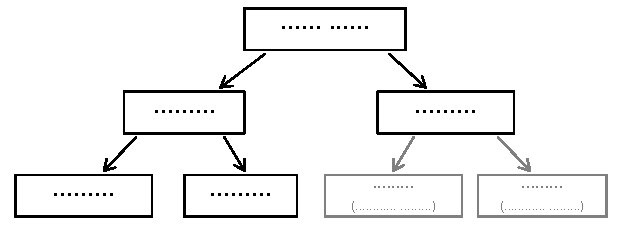
\includegraphics[width=0.57\textwidth]{ch_intro_to_data/figures/variables/variables}
\caption{각 변수 유형별 변수 분해}
\label{variables}
\end{figure}


마지막으로... \var{smoking\_\hspace{0.3mm}ban} 변수를 생각해 보자.
이 변수는 군별로 금연 유형을 기술하는데, \resp{없음(none)}, \resp{부분금지(partial)}, \resp{전면금지(comprehensive)} 값을 갖는다. 하이브리드 변수로 볼 수 있다: 범주형 변수지만, 각 수준은 자연적인 순위를 갖는다.
이러한 특성을 갖는 변수를 \term{서수형(ordinal)} 변수라고 부른다.
분석을 단순화하기 위해서, 이 책에서 어떤 서수형 변수도 범주형 변수로 처리한다.


\begin{example}{통계학 과목 수강한 학생에 관한 데이터가 수집되었다. 각 학생에 대해 변수 세개가 기록되어 있다: 형제자매 숫자, 학생 키, 이전에 통계학 과목 수강여부. 각 변수를 연속 숫자형, 이산 숫자형, 범주형으로 구분하라.}
형제자매 숫자와 학생 키는 숫자형 변수를 나타낸다.
왜냐하면, 형제 자매 숫자는 셈(count)으로 이산형이다. 신장은 연속적으로 변해서 연속형 숫자 변수다.
마지막 변수는 학생을 두 범주로 구분한다 -- 통계학 과목을 수강했던 학생과 그렇지 않은 학생 -- 이 과정을 통해서 변수가 범주형이 된다.
\end{example}

\begin{exercise} \index{데이터(data)!뇌졸증}
~\ref{basicExampleOfStentsAndStrokes}에 있는 스텐츠 조사로부터  \var{group} 과 (30일) \var{outcome} 변수를 고려해보자.
이 변수는 숫자형 변수일까요, 범주형 변수일까요?\footnote{각 변수마다 단지 두가지 가능한 값이 있고,
각 경우에 대해 범주를 기술한다. 그래서 각각은 범주형 변수가 된다.}
\end{exercise}

\subsection{변수 사이 관계}
\label{variableRelations}

연구자들은 두개 혹은 그 이상 변수 사이 관계를 찾으려는 동기로 분석을 시작한다.
사회 과학자는 다음 질문에 대답하고 싶을 것이다:

\begin{enumerate}
\setlength{\itemsep}{0mm}
\item[(1)]\label{fedSpendingPovertyQuestion} 
높은 빈곤율을 갖는 시군에서 연방정부지출은 평균적으로 더 높은가 혹은 낮은가?
\item[(2)]\label{ownershipMultiUnitQuestion} 
만약 자가소유가 특정 시군에서 전국평균보다 낮다면,
해당 시군에 다가구 비율이 전국평균을 상회할까 혹은 하회할까?
\item[(3)]\label{isAverageIncomeAssociatedWithSmokingBans} 
더 높은 평균소득을 올리는 시군은 어딜까: 금연정책을 시행하는 시군 혹은 그렇지 않은 시군일까?
\end{enumerate}

이러한 질문에 대답하기 위해서, 표~\ref{countyDF}에 나타난 \data{county} 데이터셋 같은 데이터가 수집되어 한다.
요약 통계량을 조사를 통해 시군별로 상기 3개 질문에 대한 통찰을 얻을 수 있다.
추가적으로, 그래프를 사용해서 데이터를 시각적으로 요약할 수 있고, 상기 질문에 답하는데도 유용하다.

\indexthis{산점도}{scatterplot}는 두 숫자형 변수 사이에 관계를 조사하는데 사용되는 일종의 그래프다.
그림~\ref{county_fed_spendVsPoverty}은 \var{fed\_\hspace{0.3mm}spend} 변수와 \var{poverty} 변수를 비교한다.
플롯에 각 점은 단일 시군을 나타낸다.
예를 들어, 부각된 점은 \data{county} 데이터셋에서 1088 군에 상응한다: 켄터키주 오우슬리 군(Owsley County, Kentucky)으로 빈곤율이 41.5\%이고 연방정부지출은 일인당 \$21.50 달러다.
산점도를 통해서 두 변수 사이에 관계를 유추할 수 있다: 높은 빈곤율을 갖는 시군이 약간 더 높은 연방정부지출을 받는 경향이 있다. 다양한 생각을 내서 이런 관계가 존재하는 이유는 무엇이고 각 아이디어를 조사해서 어느 것이 가장 합리적인 설명인지 판단해보자.

\begin{figure}
\centering
\includegraphics[width=0.8\textwidth]{ch_intro_to_data/figures/county_fed_spendVsPoverty/county_fed_spendVsPoverty}
\caption{\var{\var{poverty} 빈곤율에 대한 fed\_\hspace{0.3mm}spend} 연방정부지출을 보여주는 산점도.
41.5\% 빈곤율과 1인당 \$21.50 연방정부지출 정보를 갖는 켄터키주 오우슬리군이 부각되어 있다.}
\label{county_fed_spendVsPoverty}
\end{figure}

\begin{exercise}
표~\vref{email50Variables}에 기술된 \data{email50} 데이터셋에 있는 변수를 조사하라.
본인 관심을 사로잡는 변수 사이 관계에 관해서 질문 2개를 만들어보세요.
\footnote{두 예제 질문: (1) 전자우편에 줄바꿈이 많으면 전자우편에 문자가 많은 경향이 있다고 직관적으로 볼 수 있다: 이것이 사실일까? (2) 전자우편 형식이 일반 텍스트면 스팸 메시지 혹은 HTML 이면 스팸메시지라는 연관관계가 있을까?}
\end{exercise}

\var{fed\_\hspace{0.3mm}spend} 와 \var{poverty} 변수는 연관(associated)되었다고 하는데 플롯을 통해 식별할 수 있는 패턴이 보이기 때문이다. 두 변수가 서로에 어떤 연관을 보일 때, 두 변수를 \term{연관(associated)} 변수라고 부른다. 연관된 변수는 또한 \term{종속(dependent)} 변수라고 불리기도 하고 역도 또한 같다.


\begin{example}{상기 예제는 자가소유와 다가구 건축물(예를 들면, 콘도, 아파트) 비율 관계를 조사해서 
그림~\ref{multiunitsVsOwnership}에 산점도를 사용해서 시각화했다. 두 변수는 연관되었는가?}
다가구 건축물에서 구성단위 분율이 크면 클수록 자가소유비율이 낮아지는 것으로 나타난다.
두 변수 사이에 일정 관계가 있기 때문에, 두 변수는 연관되어 있다.
\end{example}


\begin{figure}
   \centering
   \includegraphics[width=0.8\textwidth]{ch_intro_to_data/figures/multiunitsVsOwnership/multiunitsVsOwnership}
   \caption{전체 3,143 시군에 대한 다가구 건축물 구성 비율과 자가소유비율 사이의 산점도.
   흥미있는 독자는 추가적으로 세번째 변수(군 인구)를 추가한 플롯 이미지를 \oiRedirect{textbook-homeownership_vs_multi_unit_structures}{www.openintro.org/stat/down/MHP.png}에 확인할 수 있다.}
   \label{multiunitsVsOwnership}
\end{figure}

그림~\ref{multiunitsVsOwnership}에 우하향 경향이 보이기 때문에 -- 다가구 건축물 대한 비율이 높은 시군이 더 낮은 자가소유와 연관되어 있다 -- 두 변수는 \termsub{음의 연관}{negative association}성을 갖는다고 한다. 
\term{양의 연관}은 그림~\ref{county_fed_spendVsPoverty}에  \var{poverty} 와 \var{fed\_\hspace{0.3mm}spend} 변수 관계에 나타나 있다.  여기서 더 높은 빈곤율을 갖는 시군이 일인당 더 많은 정부지출지원을 받는 경향이 있다.

만약 두 변수가 연관되지 않는다면, 두 변수는 \term{독립(independent)}적 이라고 한다.
즉, 두 변수 사이에 명백한 관계가 없다면, 두 변수는 독립이다.

\begin{termBox}{\tBoxTitle{연관되거나 독립적이거나 하지만 둘다는 안된다}
변수 한쌍은 어떤 방식으로 (연관) 관련이 있거나 (독립적) 없다.
어떤 변수 쌍도 연관되고 독립적이지는 않다.}
\end{termBox}

\index{데이터!시군|)}

%%%%%
\section[Overview of data collection principles]{데이터 수집 원칙 개요 \sectionvideohref{youtube-2N_bkiyTiXU&list=PLkIselvEzpM6pZ76FD3NoCvvgkj_p-dE8}}
\label{overviewOfDataCollectionPrinciples}

\index{표본|(}
\index{모집단|(}

과학적인 연구를 수행하는 첫번째 단계는 조사할 연구주제 혹은 문제을 식별하는 것이다.
명확히 설정된 연구문제는 어떤 주제 혹은 사례가 연구되어야 하고, 어떤 변수가 중요한지 식별하는데 도움을 준다.
또한 데이터를 \emph{어떻게(how)} 수집할지도 중요하다. 그렇게 함으로써 데이터에 신뢰성이 높아지고 연구 목적을 달성하는데 도움이 된다.

\subsection{모집단과 표본}
\label{populationsAndSamples}

다음 세가지 연구문제를 생각해보자:

\begin{enumerate}
\setlength{\itemsep}{0mm}
\item 대서양 황새치(swordfish)에 포함된 평균 수은 함량은 얼마인가?

\item\label{timeToGraduationQuestionForUCLAStudents} 
지난 5년간 듀크대학생이 학위를 얻는데 평균적으로 걸리는 기간은 얼마인가?
\item\label{identifyPopulationOfStentStudy} 
신약은 심각한 심장질환을 가진 환자의 사망률을 낮추는가?
\end{enumerate}

각 연구문제는 목표 \term{모집단}과 관련되어 있다.
첫번째 문제는 목표 모집단이 대서양에 있는 모든 황새치가 되고 각 물고기는 한가지 사례를 대표한다.
종종 모집단에 있는 모든 사례에 대한 데이터를 수집하는 것은 비용이 너무 많이 든다.
대신에, 표본을 수집한다. \term{표본}은 사례의 일부이며 종종 모집단의 작은 일부분이다.
예를 들어, 모집단에서 청새치 60 마리 (혹은 다른 숫자)가 선택되면 표본 데이터를 사용해서 모집단 평균을 추정하고 연구문제에 답을 구한다.


\begin{exercise} \label{identifyingThePopulationForTwoQuestionsInPopAndSampSubsection}
상기 두번째 세번째 문제 대해서, 목표 모집단과 개별 사례가 나타내는 것을 식별하세요.
\footnote{(\ref{timeToGraduationQuestionForUCLAStudents}) 
두번째 질문은 단지 학위를 마친 대학생에게만 관련됨에 주목한다; 학위를 끝마치지 못한 대학생 정보를 사용해서 평균을 계산할 수 없다.
그래서 단지 지난 5년간 졸업한 대학생만이 고려중인 모집단에 사례를 대표하게 된다.
그런 대학생만  개별 사례를 대표하게 된다. (\ref{identifyPopulationOfStentStudy}) 
심각한 심장 질환을 가진 환자가 사례를 대표하게 된다. 모집단에는 심각한 심장 질환을 갖는 모든 환자가 포함된다.}
\end{exercise}


\subsection{일화적 증거(Anecdotal evidence)}
\label{anecdotalEvidenceSubsection}

상기 세가지 연구문제에 대한 가능한 응답을 생각해보자:

\begin{enumerate}
\item 청새치를 먹어서 수은에 중독된 뉴스에 한 남자가 나왔다. 그래서 청새치에 평균 수은 함량은 치명적으로 매우 높음에 틀림없다.

\item\label{iKnowThreeStudentsWhoTookMoreThan7YearsToGraduateAtDuke} 
저자가 듀크 대학을 졸업하는데 7년 이상 걸린 두 대학원생을 만났다. 그래서 다른 대학보다 듀크 대학을 졸업하는데 더 오래 걸림이 틀림없다.
\item\label{myFriendsDadDiedAfterSulphinpyrazon} 
내 친구 아버지가 심장마비가 생겼고, 새로운 심장질환 약을 처방받은 후에 돌아가셨다. 그래서 신약은 약효가 없음에 틀림없다.
\end{enumerate}

결론 각각은 데이터에 기반하고 있다. 하지만, 두가지 문제점이 있다.
첫째, 데이터가 단지 하나 혹은 두가지 사례만 대표한다.
둘째, 그리고 좀더 중요하게 해당 사례가 모집단을 실제 대표하는지 명확하지가 않다.
이러한 무계획적인 방식으로 수집된 데이터를 \term{일화적 증거}라고 부른다.

\setlength{\captionwidth}{\textwidth-80mm}
\begin{figure}
\centering
\hspace{8mm}\includegraphics[width=55mm]{ch_intro_to_data/figures/mnWinter/mnWinter}\hspace{4mm}
\begin{minipage}[b]{\textwidth - 80mm}
   \caption[anecdotal evidence]{
   2010년 2월 일부 미디어 전문가가 나서서 대형 눈폭풍 하나를 지구 온난화에 대한 적법한 증거로 인용했다.
   코메디언 존 스튜워트(Jon Stweart)는 ``특정 군에 한 지역에 폭풍 하나." 라는 점을 지적했다.
   \label{mnWinter}}
\end{minipage}
\end{figure}
\setlength{\captionwidth}{\mycaptionwidth}

\begin{termBox}{\tBoxTitle{일화적 증거}
무계획적인 방식으로 수집된 데이터에 주의하라. 그러한 증거는 사실이고 입증할 수 있지만, 흔치 않은 사례만 대표할 수 있다.}
\end{termBox}

일화적 증거는 통상 흔치 않는 사례로 구성되는데, 두드러진 특성에 기반해서 회상되는 것이다.
예를 들어, 4년만에 졸업한 학생 6명보다 7년 걸려 졸업한 두명을 좀더 기억할 듯 하다.
가장 특이한 사례를 살펴보는 대신에, 모집단을 대표하는 많은 표본 사례를 조사해야 한다.

\subsection{모집단으로부터 표본추출}

\index{표본!임의 표본|(}

대학생 표본을 수집해서 지난 5년간 듀크 대학생에 대한 졸업기간을 추정해보자.
지난 5년간 모든 졸업생이 \emph{모집단}\index{모집단}을 대표하고, 검토를 위해서 선정된 대학생을
총괄해서 \emph{표본}\index{표본}이라고 부른다.
일반적으로 항상 모집단에서 표본을 \emph{무작위로(randomly)} 선택하려고 한다.
가장 기본적인 임의 표본 선정 유형은 추첨 진행방식과 동등하다.
예를 들어, 대학생을 선택할 때 추첨표에 각 학생 이름을 적고 100 장을 뽑는다.
뽑힌 이름이 무작위로 추출한 학생 100명 표본을 대표한다.

\begin{figure}[ht]
\centering
\includegraphics[width=0.47\textwidth]{ch_intro_to_data/figures/popToSample/popToSampleGraduates}
\caption{상기 도표에서, 졸업생 5명이 모집단에서 무작위로 뽑혀 표본에 포함된다.}
\label{popToSampleGraduates}
\end{figure}

표본을 왜 무작위로 뽑을까요? 손으로 표본을 뽑으면 안되나요? 다음 시나리오를 생각해보자.

\begin{example}{우연히 영양학을 전공하는 학생에게 연구조사를 위해서 졸업생 몇명을 선정해 달라고 요청한다고 가정하자.
본인이 판단하기에 어떤 학생 유형을 선정할 것 같은가? 이러한 표본이 모든 졸업생을 대표할 것으로 생각합니까?}
아마도, 건강과 연관된 전공분야에서 균형이 맞지 않는 숫자의 졸업생을 선택할 것이다.
혹은 아마도 모집단을 잘 대표하게 표본을 추출할 수도 있다.
설사 해당 \emph{편의(biased)}가 의도적이지 않거나 식별하기 어렵더라도  수작업으로 표본을 추출할 때, \emph{편의(biased)}된 표본을 추출할 위험을 감수하게 된다.
\end{example}

\begin{figure}
\centering
\includegraphics[width=0.47\textwidth]{ch_intro_to_data/figures/popToSample/popToSubSampleGraduates}
\caption{동일하게 모든 졸업생으로부터 표본을 추출하는 대신에, 영양학 전공 학생은 우연히 건강 관련 전공자를 불균형하게 표본으로 추출할 수 있다.}
\label{popToSubSampleGraduates}
\end{figure}

만약 누군가 표본에 어떤 졸업생이 포함되어야 하는지 정확하게 선택해서 뽑을 수 있다면, 표본이 해당 사람의 관심에 치우치는 것도 완전히 가능한데, 이것은 완전히 고의가 아닐 수 있다. 이렇게 하면 표본에 \term{편의}가 들어오게 된다. 무작위 표본추출은 이러한 문제를 푸는데 도움이 된다. 가장 기본적인 임의표본은  \term{단순 임의 표본}으로 불리며 사례를 선택하는데 추첨표를 사용하는 것과 동등하다.
모집단 각 사례는 표본에 포함될 동일한 확률을 갖고 표본에 있는 사례간에는 어떤 암묵적인 연관관계도 없다는 것을 의미한다.

\APVersion{종종 단순임의표본을 구현이 어려워서 대체 방법이 도움이 된다.
\term{계통 추출법}이 한 대체법이 되고, 고정된 숫자 예를 들어 매번 10번째 사례 마다 표본을 추출한다.
이러한 접근법은 쉽게 사람으로 인한 편의에 노출되지 않는 매커니즘을 사용하기 때문에, 
종종 상당한 대표성을 갖는 표본을 산출한다. 
이 책은 표본 추출에만 집중하는데 계통추출법을 사용하는 것은 일반적이지 않고, 문맥에 따른 부가적인 고려가 필요하기 때문이다.}{}

단순임의표본을 취하는 행위가 편의를 최소화하는데 도움을 주지만, 편의는 다른 방식으로 불쑥 나타난다.
예를 들어 설문조사를 위해 사람을 임의로 뽑을 때 조차도, \term{무응답} \index{표본!무응답|textbf}이 높다면 주의를 기울여야 한다.
예를 들어, 설문조사에 무작위로 뽑힌 30\% 사라만 응답했다면,
결과가 전체 모집단에 \term{대표성}을 갖는지 명확하지 않다. 이러한 \term{무응답 편의} \index{표본!무응답 편의|textbf}가 결과를 
왜곡할 수 있다.

\begin{figure}[h]
\centering
\includegraphics[width=0.5\textwidth]{ch_intro_to_data/figures/popToSample/surveySample}
\caption{
무응답 가능성 때문에, 설문조사는 모집단 내부에서 특정 집단에만 도달하게 된다.
이 문제를 완전히 고치는 것은 어렵고, 종종 불가능하다.}
\label{surveySample}
\end{figure}

또 다른 흔히 빠지는 함정이 \term{편의 표본}\index{표본!편의 표본}으로 쉽게 접근할 수 있는 개인이 표본에 좀더 포함될 듯 하다.
예를 들어, 만약 정치 설문조사가 브롱크스 행인을 대상으로 수행된다면, 뉴욕시 전체를 대표할 것 같지는 않다.
편의 표본이 어떤 하위-모집단을 대표하는지 분간하는 것이 종종 어렵다.

\begin{exercise}
웹사이트를 통해서 쉽게 제품, 판매자, 회사에 대한 평가점수에 접근할 수 있다.
이러한 평점은 평가점수를 제공하려고 노력한 사람들에 기반해서 매겨졌다.
만약 제품에 대한 50\% 온라인 사용후기가 부정적이라면, 이러한 사실이 구매자 50\%가 해당 제품에 불만족한다고 보십니까?
\footnote{대답은 다양할 수 있다.
우리 스스로 일화적 경험으로부터,
기대한대로 동작하는 제품에 대해서 격찬하기 보다는 기대에 떨어지는 제품에 대해서 못마땅하게 과장되게 사람들이 말하는 경향이 있다고 믿는다. 이러한 이유로, 아마존 같은 사이트에 올라온 제품 평점에 음의 편향이 있다고 의심할만 하다.
하지만, 본인의 경험이 대표성을 갖지 않을 수 있기 때문에, 마음을 항상 열어놓자.}
\end{exercise}

\index{표본!임의 표본|)}
\index{모집단|)}
\index{표본|)}

\subsection{설명 변수와 반응 변수}
\label{explanatoryAndResponse}

\index{데이터!시군|(}

\data{county} 데이터셋에 대해 ~\pageref{fedSpendingPovertyQuestion} 페이지에 나온 다음 질문을 생각해 보자.

\begin{enumerate}
\item[(1)] 
	높은 빈곤율을 갖는 시군에서 연방정부지출은 평균적으로 더 높은가 혹은 낮은가?
\end{enumerate}

만약 빈곤이 해당 군 지출에 영향을 미친다고 의심하면, 빈곤은 \term{설명} 변수가 되고 연방정부지출은 관계에 있어 \term{반응} 변수가 된다 \footnote{
종종 설명 변수는 \term{독립} 변수로 불리고, 반응 변수는 \term{종속} 변수로 불린다.
하지만, 이렇게 되면 혼동스러울 수 있는데 이유는 변수 \emph{한쌍}이 독립적 혹은 종속적일 수 있기 때문이다. 이러한 사유로 이런 단어를 회피한다.} 
만약 변수가 많다면, 이들 중 일부를 설명변수로 간주하는 것도 가능할 수 있다.

\begin{tipBox}{\tipBoxTitle{설명 변수와 반응 변수}

변수 한쌍에서 설명 변수를 식별하기 위해서, 둘 중에 어느 것이 다른 것에 영향을 주는지 식별하고 적절한 분석을 계획하라.

\hspace{10mm}\includegraphics[height=0.34in]{ch_intro_to_data/figures/expResp/expResp}}
\end{tipBox}

\begin{caution}{연관성이 인과성을 함축하지는 않는다}{
\emph{설명변수}와 \emph{반응변수}로 표식을 했다는 것이 두 변수 사이 관계가 실제로 인과성이 있다는 것을 담보하지는 않는다. 설사 두 변수 사이에 연관이 확인되어도 그렇다. 어느 변수가 다른 변수에 영향을 미치는지 용의점을 추적하는데만 표식을 사용한다.}
\end{caution}

일부 설명변수와 반응변수가 없는 경우가 있다. 페이지~\pageref{ownershipMultiUnitQuestion}에서 다음 질문을 생각해보자:

\begin{enumerate}
\item[(2)]
    만약 특정 군에서 자가소유가 전국 평균보다 낮다면, 다가구 건축물 비율이 전국 평균을 상회할까요 아니면 하회할까요?
\end{enumerate}

어느 변수가 설명변수이며, 반응변수인지 판단하기가 어렵다. 즉, 방향성이 애매모호하다. 그래서 설명 혹은 반응 표식을 여기서는 제시할 수는 없다.

\index{데이터!군|)}

\subsection{관측연구와 실험 소개}

데이터 수집에 두가지 유형이 있다: 관측연구와 실험.

데이터가 생성되는 방식에 직접적인 지장을 받지 않는 방식으로 데이터를 연구원이 수집할 때 \term{관측연구}를 수행한다.
예를 들어, 왜 특정 질병이 진행되는지 조사하기 위해서, 과학연구원은 설문조사를 경유해 정보를 수집하고, 진료 및 회사 기록을 검토하고, 
유사성 있는 다수 \term{코호트} 환자를 추적한다.
이러한 상황에서 과학연구원은 단지 발생된 데이터를 관측한다.
일반적으로, 관측연구는 변수사이에 자연적으로 발생하는 연관 증거를 제공할 수 있지만, 그 자체로 인과관계를 제시할 수는 없다.

연구원이 인과관계 가능성을 조사하려면, \term{실험}을 수행한다.
대체로 설병변수와 반응변수 모두 있다.
예를 들어, 약을 투여하는 것이 다음해에 심장마비 환자의 사망율을 줄일 수 있는지 의심할 수 있다.
설명변수와 반응변수 사이에 인과관계가 정말 있는지 검사하기 위해서, 연구원은 개인 표본을 수집하고 그룹으로 나눈다.
각 그룹에 개인은 처리군(treatment)에 \emph{배정}된다. 개인이 무작위로 그룹에 배정될 때, 해당 실험을 \term{무작위 실험}이라고 부른다.
예를 들어, 의약 시험에 각 심장마비 환자를 아마도 동전던지기를 통해서 두 그룹중에 한 곳에 임의로 배정할 수 있다:
첫번째 그룹은 \term{위약} (placebo, 거짓처방)을 처방받고, 두번째 그룹은 약물을 처방받는다.
실험의 또다른 예제로 ~\ref{basicExampleOfStentsAndStrokes}에 사례연구를 참조한다. 하지만 해당 조사는 위약을 사용하지는 않는다.



\begin{tipBox}{\tipBoxTitle{연관 $\neq$ 인과}
일반적으로 연관(assocaition)은 인과(causation)를 함축하지는 않는다. 그리고 인과는 무작위 실험으로만 추론될 수 있다.}
\end{tipBox}


%%%%%
\section[Observational studies and sampling strategies]{관측연구와 표본추출 전략 \sectionvideohref{youtube-n1xSeGPGQEg&list=PLkIselvEzpM6pZ76FD3NoCvvgkj_p-dE8}}

\subsection{관측연구}

일반적으로, 관측연구에 있어 데이터는 일어난 것을 모니터링하면서만 수집된다.
반면에, 연구 주요 설명변수를 연구원이 각 대상마다 배정할 것을 실험에서는 요구한다.

실험에 근거해서 인과결론을 내리는 것은 합리적이다. 하지만,
관측연구에 근거해서 동일한 인과 결론을 내리는 것은 겉보기와 달리 위험하고 추천되지 않는다.
그래서, 관측연구는 일반적으로 연관만 보이는데 충분하다.


\begin{exercise} \label{sunscreenLurkingExample}
관측연구가 선크림 사용과 피부암을 추적했다고 가정하자. 그리고 선크림을 더 많이 사용하면 할수록,
사람들이 더 피부암에 걸릴 것 같다는 것이 밝혀졌다. 이것이 선크림이 피부암에 \emph{원인}이 된다는 것을 의미할까?
\footnote{아니다. 설명으로 문단과 이어진 예제를 살펴보라.}
\end{exercise}

일부 이전 연구를 통해 선크림을 사용하면 피부암 위험을 실제로 줄여준다고 알려졌다.
그래서 아마도 선크림 사용과 피부암 사이에 가상의 연관(hypothetical association)을 설명하는 또다른 변수가 있을 수 있다.
빠진 중요한 정보 조각이 일광노출이다.
누군가 하루종일 태양에 노출된다면, 선크림을 좀더 사용할 것 \emph{같고} 더 피부암에 걸릴 것 같다.
일광노출이 단순 조사에서 고려되지 못했다.

\begin{center}
\includegraphics[height=1.0in]{ch_intro_to_data/figures/variables/sunCausesCancer}
\end{center}
% Some studies:
% http://www.sciencedirect.com/science/article/pii/S0140673698121682
% http://archderm.ama-assn.org/cgi/content/abstract/122/5/537
% Study with a similar scenario to that described here:
% http://onlinelibrary.wiley.com/doi/10.1002/ijc.22745/full

일광노출을 \term{교락변수}라고 부르고, \footnote{또한 \term{잠복변수}(lurking variable), \term{교락요인}(confounding factor), 혹은 \term{교락요인}(confounder)이라고 부른다.} 설명변수와 반응변수 모두와 상관된 변수다.
관측연구로부터 도출된 인과결론을 정당화하는 방법은 교락변수를 철저히 찾는 것이지만, 
모든 교락변수가 측정되거나 조사될 수 있다는 보장은 없다.

동일한 방식으로, \data{county} 데이터셋은 교락변수를 갖는 관측연구다. 그리고 인과결론을 도출하는데 데이터가 쉽게 사용될 수는 없다.

\begin{exercise}
그림~\ref{multiunitsVsOwnership}에 자가소유비율과 다가구 건축물 비율 사이에 부의 연관성이 보인다.
하지만, 두 변수 사이에 인과관계가 존재한다고 결론 내리는 것은 합리적이지 못하다.
그림~\ref{multiunitsVsOwnership}에 나타난 시각적 관계를 설명하는 하나 혹은 그 이상 다른 변수를 제시하세요}.
\footnote{정답은 다양하다. 인구밀도가 중요할 수도 있다. 만약 특정 군이 매우 밀도가 높다면, 주민 상당수가 다가구 건축물에 살아야만 된다. 부가적으로 높은 밀도는 부동산 가치를 높여서 다수 주민이 자가소유건물을 갖지 못하게 할 것 같다.}
\end{exercise}

관측연구는 두가지 형태가 있다: 전향적 연구(prospective studies)와 후향적 연구(retrospective studies).
\term{전향적 연구}는 개인을 식별하고 사건이 진행됨에 따라 정보를 수집해 나간다.
예를 들어, 의학 연구원은 수년간에 걸쳐 한 집단의 유사한 개인을 식별하고 추적하여 암위험에 있어 행동의 가능한 영향을 평가한다.
이러한 유형을 갖는 연구 한 사례가 간호사 건강연구(The Nurses' Health Study)로 1976년 시작해서 1989년까지 진행되었다.\footnote{\oiRedirect{textbook-channing_nurse_study}{www.channing.harvard.edu/nhs}} 
이 전향연구는 등록된 간호사를 모집하고 나서 설문지를 사용해서 데이터를 수집했다.
\termsub{후향적 연구}{retrospective studies}는 사건이 발생한 후에 데이터를 수집한다. 즉,
연구원이 의료기록을 통해서 지난 사건을 검토할 수 있다. \data{county} 같은 일부 데이터는 전향적 이며 후향적 방식으로 시집된 변수를 모두 포함하고 있다. 지방정부는 전향적으로 사건이 전개되어가면 일부 변수를 수집(예를 들어, 소매)하는 반면에,
연방정부는 후향적으로 2010년 인구총조사 기간동안 다른 변수를 수집했다 (예를 들어, 군 인구).

\subsection{네가지 표집 방법 (특별 주제)}
\label{fourSamplingMethods}
\label{threeSamplingMethods}

거의 모든 통계적 방법은 암묵적 임의성(implied randomness) 개념에 기초하고 있다.
만약 관측된 데이터가 모집단으로부터 임의 구조 아래에서 수집되지 않는다면,
이런 통계적 방법-- 추정값와 추정값과 연관된 오차 --은 신뢰성이 없다.
여기서 네가지 임의 표본추출 기법을 고려한다: 단순표집(simple), 층화표집(stratified), 군집표집(cluster), 다단계표집(multistage).
 그림~\ref{simple_stratified}와 ~\ref{cluster_multistage}에 네가지 기법을 시각적으로 표현했다.


\begin{figure}
\centering
\includegraphics[width=\textwidth]{ch_intro_to_data/figures/samplingMethodsFigure/simple_stratified}
\caption{단순임의표집\index{표본!단순임의표집}과 층화표집\index{표본!층화표집} 예제. 상단 그림에서는 단순임의표집을 사용해서 18개 사례를 임의로 뽑았다.
하단 그림에서는 층화표집이 사용되었다: 사례를 층(strata)으로 그룹으로 만들고 나서 \mbox{각 층}마다 내부적으로 단순임의표집을 사용했다.}
\label{simple_stratified}
\end{figure}

\termsub{단순임의표집}{표본!단순임의보집}은 아마도 가장 직관적인 임의추출방법이다.
메이저 리그 야구(Major League Baseball, MLB) 선수 연봉을 생각해보자.
여기서 선수 각각은 리그에 속한 30개팀 중 한팀의 일원이다.
야구선수 120명을 임의 표본으로 뽑아 2010 시즌 연봉 정보를 수집하려면,
제비쪽지에 해당 시즌 야구선수 828명 명단을 적고, 뽑기함에 제비쪽지를 넣고, 선수명단이 잘 섞일 때까지 뽑기함을 흔들고 나서
표본 야구선수 120명을 뽑을 때까지 제비뽑기를 진행한다.
일반적으로, 만약 모집단에서 사례 각각이 최종 표본에 포함될 동일한 확률을 \emph{갖고} 특정 사례가 표본에 포함된다는 것을 아는 것이 어떤 다른 사례가 포함될지에 관한 유용한 정보를 제공하지 않는다면, 해당 표본을 ``단순임의표본(simple random sample)''이라고 부른다.


\termsub{층화표집}{표본!층화표집}은 분할정복(divide and conquer) 표집 전략이다.
모집단을 \term{층}\index{표본!층|textbf}으로 불리는 집단으로 분할한다.
층은 유사한 사례를 함께 무리짓고 나서, 두번째 표집 방법, 일반적으로 단순임의표집을 각 층에 사용한다.
프로야구 연봉 예제에서, 팀이 층을 대표할 수 있다. 왜냐하면 일부 팀이 돈을 많이 갖고 있기 때문이다(최대 4배).
그러면, 무작위로 각 팀마다 선수 4명을 임의로 추출하여 전체 120명을 뽑을 수 있다.


층화표집이 특히 유용할 때는 각 층에 사례가 관심있는 결과에 비추어 매우 유사할 때다.
단점은 층화표본 데이터를 분석하는 것이 단순임의표본에서 나온 데이터를 분석하는 것보다 더 복잡한 작업이라는 것이다.
층화표집을 사용해서 수집된 데이터를 분석하기 위해서는 이 책에서 소개된 분석 방법을 확장될 필요가 있다.

\begin{example}{각 층 내부에 사례를 매우 유사하게 만드는 것이 왜 좋을까?}
만약 사례가 매우 유사하다면, 층내 하위모집단에 대해서 좀더 안정된 추정값을 얻을 수 있다.
각 하위모집단에 대한 이러한 향상된 추정값을 통해 전체 모집단에 대한 신뢰성있는 추정값을 만들어 낼 수 있다.
\end{example}


\termsub{군집표본}{표본!군집표본}에서, 모집단을 \termsub{군집}{표본!군집}으로 불리는 다수 집단으로 쪼갠다.
그리고 나서, 정행진 군집수를 표집하고 표본에는 각 군집으로부터 모든 관측점을 포함한다.
\termsub{다단계 표본}{표본!다단계 표본}은 군집표본과 같지만, 각 군집에 모든 관측점을 선택하기 보다는
선택된 각 군집내부에서 임의 표본을 추출한다. %Multistage sampling is similar to stratified sampling in its process, except that stratified sampling requires observations be sampled from \emph{every} stratum.

\begin{figure}
\centering
\includegraphics[width=\textwidth]{ch_intro_to_data/figures/samplingMethodsFigure/cluster_multistage}
\caption{
군집표집\index{표본!군집 표집}과 다단계표집\index{표본!다단계 표집} 예제.
상단 그림에서 군집표집이 사용되었다. 여기서 데이터가 9개 군집으로 나누고, 이 군집중에서 세개를 표본으로 선택했고,
세 군집에 있는 모든 관측점이 최종표본에 포함됐다. 
아래 그림에서 다단계표집이 사용되었다.
선택된 군집중에서 최종 표본에 포함되려면 각 군집의 일부를 무작위로 선택한다는 면에서 군집표집과 다르다.}
\label{cluster_multistage}
\end{figure}

때때로, 군집표집과 다단계표집이 대안 표집기법보다 더 경제적일 수 있다.
또한, 층화표집과 달리, 군집 내부에 사례마다 변동성이 상당하지만, 근집 자체는 다른 것과 그다지 차이가 없을 때 이러한 접근법이 가장 도움이 된다. 예를 들어, 만약 이웃이 군집을 대표한다면, 군집 혹은 다단계 표집은 이웃이 매우 다양할 때 가장 잘 동작한다.
설사 이책에 방법을 확장할 수는 있지만, 이러한 방법의 단점은 일반적으로 좀더 고급 분석기법이 요구된다는 점이다.

\begin{example}{인도네시아 농촌 열대 밀림지역에 말라리아 발병율을 추정하는데 관심이 있다고 가정하자.
해당 인도네시아 정글 지역에 마을이 30개가 있는데, 각 마을을 옆 마을과 유사하다는 것을 알게되었다.
목적은 말라리아에 대해 150 명을 테스트하는 것이다. 어떠한 표집방법이 적용되어야 하는가?}
단순임의표본은 모든 30개 마을에서 개인 표본을 뽑을 듯 한데 데이터 수집에 비용이 엄청 많이 들 수 있다.
층화표집은 도전과제가 될 수 있는데 유사한 개인을 층화하는 방법이 명확하지 않다.
하지만, 군집표집 혹은 다단계표집은 매우 좋은 아이디어처럼 보인다.
만약 다단계표집을 사용하기로 결정한다면, 무작위로 마을 반을 선택하고 나서 각 마을마다 10명을 무작으로 선택한다.
이렇게 하면 아마도 단순임의표본과 비교해서 데이터 수집 비용이 상당히 줄 수 있으면서도 여전히 신뢰성 있는 정보를 줄 것이다.
\end{example}


%%%%%
\section[실험]{Experiments \sectionvideohref{youtube-g7JGe_ykB3I&list=PLkIselvEzpM6pZ76FD3NoCvvgkj_p-dE8}}
\label{experimentsSection}

연구원이 처리(treatment)를 사례에 배정하는 연구를 \termsub{실험}{experiment}이라고 부른다.
이러한 배정에 임의화(randomization)가 포함될 때, 예를 들어 동전을 던져 환자가 어떤 처리를 받을지 결정하는 것같은,
\term{임의화 실험(randomized experiment)}이라고 부른다. 두 변수 사이에 인과관계를 보여주려고 할 때 임의화 실험은 근본적으로 중요하다.

\subsection{실험계획의 원칙}
\label{experimentalDesignPrinciples}

임의화 실험은 일반적으로 네가지 원칙 아래 구성된다.

\begin{description}
\item[제어(Controlling).] 
연구원이 처리를 사례에 배정하고 집단에 다른 어떤 차이도 \term{제어}하기 위해서 최선을 다한다.
예를 들어, 환자가 알약형태 약을 복용할 때, 일부 환자는 약을 물 조금과 함께 복용하고, 다른 환자는 약을 가득찬 물 한잔과 함께 복용할 수 있다. 물 소비 효과를 제어하기 위해서, 의사가 모든 환자에게 약과 12 온스 물 한잔만 복용하도록 할 수 있다.
\item[임의화(Randomization).] 
제어할 수 없는 변수를 설명하기 위해서, 연구원이 처리집단에 환자를 임의화한다.
예를 들어, 일부 환자는 다른 환자보다 식습관 덕분에 질병에 더 걸리기 쉬울 수 있다.
환자를 처리집단과 대조집단으로 임의화하면 그러한 차이를 균등하게 할 수 있고 우연적 편향이 연구에 들어오지 못하게도 한다.
\item[반복(Replication).] 
연구원이 더 많은 사례를 관측하면 할수록, 반응변수에 설명변수 효과를 좀더 정확하게 추정할 수 있다.
단일 연구에서 충분히 큰 표본을 수집해서 \term{반복}한다. 추가적으로, 한 무리 과학자가 전체 연구를 반복해서 이전 연구결과를 확인한다.

\begin{figure}
\centering
\includegraphics[width=0.78\textwidth]{ch_intro_to_data/figures/figureShowingBlocking/figureShowingBlocking}
\caption{환자위험을 묘사하는 변수를 사용한 블로킹.
환자가 먼저 저위험 블록과 고위험 불록을 나누고 나서, 각 블록은 임의화를 사용해서 공평하게 처리집단으로 분리된다.
이 전략은 고위험과 저위험 범주 모두로부터 각 처리집단에 동일한 환자 대표성을 갖도록 확실히 한다.}
\label{figureShowingBlocking}
\end{figure}

\item[블로킹(Blocking).] 
종종 연구원이 처리가 아닌 다른 변수가 반응에 영황을 준다고 알고 있거나 의구심을 갖고 있을 수 있다.
이러한 상황에서, 먼저 개인을 이 변수에 기반해서 \term{블록}으로 무리짓고 나서 처리 집단에 각 블록내부에서 사례를 확률화한다.
이 전략은 종종 \term{블로킹}으로 불린다. 예를 들어,
만약 심장마비에 대한 약효를 살펴본다면, 먼저 연구에 환자를 저위험 블록과 고위험 블록으로 나누고 나서 
그림~\ref{figureShowingBlocking}에 나와있듯이, 무작위로 각 블록에서 환자 절반을 대조집단에 다른 환자 절반을 치료집단에 배정한다.
이 전략은 각 처리집단에 동일한 숫자의 저위험과 고위험 환자를 갖도록 확실히 한다.
\end{description}

첫 세가지 실험계획 원칙을 어떤 연구에도 포함하는 것이 중요하다.
이 책에서는 그런 실험에서 나온 데이터를 분석하는데 적용가능한 방법을 기술한다.
블로킹은 다소 좀더 고급 기법으로 이 책에 나온 통계적 방법을 확장해서 블로킹을 사용해 수집된 자료를 분석한다.

\subsection{인간 실험에 편향 줄이기}
\label{biasInHumanExperiments}

임의화 실험이 데이터 수집에 대한 황금률이지만, 모든 사례에 불편향 측면을 인관관계에 보장하지는 못한다.
인간 실험이 완벽한 예제로서 편향이 의도하지 않았는데 일어날 수 있다.
심장마비 환자를 처리하는데 신약을 사용한 연구를 다시 생각해보자.\footnote{Anturane Reinfarction Trial Research Group. 1980. Sulfinpyrazone in the prevention of sudden death after myocardial infarction. New England Journal of Medicine 302(5):250-256.}
특히 연구원은 신약이 환자 사망률을 줄였는지 알고자 한다.

해당 연구원은 임의화 실험을 설계하는데 신약 효과에 관한 인과관계를 도출하고자 하기 때문이다.
연구 지원자\footnote{인체 실험대상은 종종 \term{환자}, \term{지원자}, \term{연구 참여자}라고 불린다.}를 두 연구집단에 임의로 나누어 배치한다. 한 집단, \term{처리집단}은 신약을 처방받는다. 다른 집단, \term{대조집단}은 어떤 신약 처방도 받지 않는다.

연구에서 참여자 위치에 본인을 투영해보라.
만약 본인이 처리집단에 있다면, 도움이 기대되는 멋진 신약을 처방받을 것이다.
다른 한편으로, 또다른 집단에 있는 참여자는 신약을 받지 못하고 놀면서 기다리는데 다만 실험 참여가 사망율을 증가시키지 않기를 기대할 뿐이다. 이러한 측면은 실제로 두가지 효과가 있다는 것을 제시한다: 관심을 둔 한 가지가 신약 효과이며, 두번째는 감정적 효과로 정량화하기가 어렵다.

연구원은 대체로 감정적 효과에는 관심이 없는데 연구에 편향을 준다.
이러한 문제를 우회하려고, 연구원은 참여자가 어느 집단에 속해있는지 알려주지 않는다.
연구원이 처리에 관한 정보를 환자에게 알려주지 않을 때, 연구를 \term{눈가림}(blind) 연구라고 한다.
하지만 문제가 하나 있다: 만약 환자가 처리를 받지 못하면, 환자를 본인이 대조집단에 있다고 알게된다.
이러한 문제에 해법이 거짓 처방을 대조집단 환자에 주는 것이다. 거짓 처방을 \term{위약}이라고 부르고,
효과적인 위약이 연구를 진정하게 눈가름으로 만드는 열쇠다. 전통적인 위약 사례가 실제 처방약처럼 만든 설탕약이다.
종종 위약을 통해 환자에서 적지만 실제 호전된 결과가 나오기도 한다.
이러한 효과를 \term{위약~효과}라는 말로 부른다.

환자만이 유일한 눈가림되어야 되는 사람은 아니다: 의사와 연구원도 우연히 연구에 편향을 줄 수 있다.
환자에 실제 처리가 주어지고 있다는 사실을 의사가 알게될 때, 의사가 무심코 위약이 처방된 환자보다 더 관심과 주의를 둘 수 있다.
일부 사례에서 측정가능한 효과를 갖는 것으로 확인된 이런 편향이 생기지 않도록 보호하기 위해서, \term{이중눈가림}(double blind) 방식을 사용한다. 환자와 상호작용하는 의사 혹은 연구원은 환자와 마찬가지로 처리를 받았는지 받지 않았는지 인식하지 못한다.
\footnote{항상 연구에 관련된 일부 연구원은 어느 환자가 어느 처리를 받고 있는지 알고 있다.
하지만, 이들 연구원은 연구 환자와 상호작용하지 못하고 누가 어느 처리를 받고 있는지 눈가림된 의료전문가에게 말하지 않는다.}

\begin{exercise}
~\ref{basicExampleOfStentsAndStrokes} 절에 연구로 되돌아가자. 연구원이 스텐트가 위험에 처한 환자의 심근경색을 줄이는데 효과가 있는지 테스트한다. 이것은 실험인가요? 이 연구는 눈가림 방식인가요?  이 연구는 이중눈가림 방식인가요?
\footnote{연구원이 환자를 처리집단에 배정했다. 그래서 해당 연구는 실험이다.
하지만, 환자는 무슨 처리를 받고 있는지 분간할 수 있다. 그래서 해당 연구는 눈가림이 아니다. 해당 연구는 이중눈가림이 될 수 없는데 연구가 눈가림 연구도도 아니기 때문이다.}
\end{exercise}


%%%%%
\section[숫자형 데이터 살펴보기]{Examining numerical data \sectionvideohref{youtube-Xm0PPtci3JE&list=PLkIselvEzpM6pZ76FD3NoCvvgkj_p-dE8}}
\label{numericalData}

이번 절에서 숫자형 변수를 탐색하고 요약하는 기법을 소개한다.
~\ref{dataBasics} 절에서 \data{email50}와 \data{county} 데이터셋이 예제로 풍부한 기회를 제공했다.
숫자형 변수 결과는 숫자로 기본적인 산술연산을 수행할 수 있다는 것을 상기하라.
예를 들어, \var{pop2010} 변수는 2010년 시군 인구를 대표하는데 숫자형이여서
두 시군 사이에 인구 차이와 비율을 분별력을 갖고 논의할 수 있다.
다른 한편으로, 지역코드와 우편번호는 숫자형이라기 보다는 범주형 변수다.


\subsection{쌍체자료(paired data) 산점도}
\label{scatterPlots}

\index{데이터!email50|(}

\term{산점도}는 두 숫자형 변수에 대한 데이터 사례별 뷰를 제공한다.
그림~\vref{county_fed_spendVsPoverty}에서 산점도를 사용해서 연방지출비용과 빈곤율이 \data{county} 데이터에서 연관되어 있는지 조사했다. 또다른 산점도는 그림~\ref{email50LinesCharacters}에 나와 있는데, \data{email50} 데이터셋에 전자우편에 줄바꿈(\var{line\_\hspace{0.3mm}breaks})과 문자 숫자(\var{num\_\hspace{0.3mm}char})를 비교했다.
임의 산점도에서 각 점은 사례 하나를 표현한다. \data{email50} 데이터셋에 50 개 사례가 있기 때문에, 
그림~\ref{email50LinesCharacters}에 점이 50개 있다.

\textC{\setlength{\captionwidth}{0.9\textwidth}}

\begin{figure}[h]
   \centering
   \includegraphics[width=0.8\textwidth]{ch_intro_to_data/figures/email50LinesCharacters/email50LinesCharacters}
   \caption{\data{email50} 데이터에 \var{line\_\hspace{0.3mm}breaks} 와 \var{num\_\hspace{0.3mm}char}에 대한 산점도.}
   \label{email50LinesCharacters}
\end{figure}

\textC{\setlength{\captionwidth}{\mycaptionwidth}}

이러한 관점에서 문자숫자를 살펴보면, 이 문단은 문자 363개로 구성되었다.
그림~\ref{email50LinesCharacters}을 살펴보면, 일부 전자우편은 말이 안될 정도로 장황한 것처럼 보인다.
좀더 조사를 하면, 장문 전자우편 대부분은 실제로 HTML 형식을 사용하는 것을 알 수 있다.
이것이 의미하는 바는 해당 전자우편 문자 대부분이 텍스트로 정보를 제공하기 보다는 전자우편 서식에 사용되었다는 것이다.


\begin{exercise}
산점도가 데이터에 관한 무엇을 밝혀냈고, 어떻게 유용하게 사용될 수 있을까?\footnote{해답은 다양하다. 산점도는 신속하게 변수와 관련된 연관성을 식별하는데 도움이 된다.즉, 연관이 단순한 추세 형태로 오는지 혹은 좀더 복잡한 관계로 나타나는지 알 수 있다.}
\end{exercise}

\index{데이터!cars|(}
\begin{example}{
변수 두개와 54개 자동차로 구성된 신차 데이터셋을 고려해보자: 자동차 가격과 자동차 중량
\footnote{출처: \oiRedirect{textbook-1993_car_data}{www.amstat.org/publications/jse/v1n1/datasets.lock.html} 데이터 일부}
자동차 가격과 중량에 대한 산점도가 그림~\ref{carsPriceVsWeight}에 나타나 있다.
이들 변수 사이 관계에 간해서 무엇을 말할 수 있을까?}
점선으로 부각되듯이 관계는 명백히 비선형이다.
이점이 지금까지 봤던 이전 산점도와 다른 면이다. 그림~\vref{county_fed_spendVsPoverty}와 그럼~\ref{email50LinesCharacters}은 매우 선형적 관계를 보여주고 있다.

\begin{figure}[h]
   \centering
   \includegraphics[width=0.8\textwidth]{ch_intro_to_data/figures/carsPriceVsWeight/carsPriceVsWeight}
   \caption{자동차 54개에 대한 \var{price} 대비 \var{weight} 산점도.}
   \label{carsPriceVsWeight}
\end{figure}
\end{example}
\index{data!cars|)}

\begin{exercise}
산점도에서 말발굽 모양을 갖는 두변수를 기술하시요.\footnote{
수직축은 뭔가 ``좋은'' 것을 표현하고 수평축은 단지 적당히 좋은 것을 표현한다.건강과 물 소비가 이러한 기술에 적합한데 물을 너무 과도하게 소비하게 되면 독성을 갖는다.}
\end{exercise}

\subsection{점그림(Dot plots)과 평균}
\label{dotPlot}

종종 두변수가 한 변수에 너무 많을 수 있다: 단지 한 변수만 관심이 있을 수 있다.
이러한 경우에 점그림이 가장 기본적인 시각적 출력을 제공한다. \term{점그림}(dot plot)은 일변수 산점도다;
50개 전자우편에서 나온 문자 숫자를 사용한 예제가 그림~\ref{emailCharactersDotPlot}에 나타나 있다.

\begin{figure}[h]
   \centering
   \includegraphics[width=\textwidth]{ch_intro_to_data/figures/emailCharactersDotPlot/emailCharactersDotPlot}
   \caption{\data{email50} 데이터셋에 대한 \var{num\_\hspace{0.3mm}char}를 점그림으로 표현.}
   \label{emailCharactersDotPlot}
\end{figure}

\begin{figure}[h]
   \centering
   \includegraphics[width=0.72\textwidth]{ch_intro_to_data/figures/emailCharactersDotPlot/emailCharactersDotPlotStacked}
   \caption{\data{email50} 데이터셋에 대한 변수 \var{num\_\hspace{0.3mm}char}의 스택 점그림(stacked dot plot).
   상기 점그림에서 값을 가장 가까운 12,000에 반올림했다.}
   \label{emailCharactersDotPlotStacked}
\end{figure}

\term{평균}(평균)은 종종 \indexthis{평균}{평균!평균(average)}(average)으로도 불리는데 데이터 \term{분포}의 중심을 측정하는 일반적인 방식이다. 50개 전자우편에 평균 문자숫자를 찾아내려면, 문자 갯수를 모두 더하고 전자우편 갯수로 나눈다.
계산 편의를 위해서, 문자 숫자는 첫단위로 표시되고 소수점 첫자리에서 반올림한다.

\begin{eqnarray}
\bar{x} = \frac{21.7 + 7.0 + \cdots + 15.8}{50} = 11.6
\label{sampleMeanEquation}
\end{eqnarray}

표본 평균은 $\bar{x}$\marginpar[\raggedright$\bar{x}$\\\footnotesize 표본\\ 평균]{\raggedright$\bar{x}$\\\footnotesize 표본\\ 평균}.로 표기한다. 문자 $x$는 관심있는 변수, \var{num\_\hspace{0.3mm}char}에 대한 일반 자리차지용도(placeholder)로 사용된다.
그리고, $x$ 위에 막대는 50개 전자우편 문자 평균 숫자가 11,600임을 전달한다.
평균을 분포의 균형점으로 간주하는 것이 유용하다. 표본 평균은 그림~\ref{emailCharactersDotPlot} 와~\ref{emailCharactersDotPlotStacked}에 삼각형으로 표현되어 있다.


\begin{termBox}{\tBoxTitle{평균}%
숫자 변수의 표본 평균은 전체 관측값을 관측수로 나눠서 계산한다:
\begin{eqnarray}
\bar{x} = \frac{x_1+x_2+\cdots+x_n}{n}
\label{meanEquation}
\end{eqnarray}
$x_1, x_2, \dots, x_n$은 $n$개 관측값을 표현한다.}
\end{termBox}\marginpar[\raggedright\vspace{-8mm}

$n$\\\footnotesize 표본 크기]{\raggedright\vspace{-8mm}

$n$\\\footnotesize 표본 크기}\vspace{-2mm}

\begin{exercise}

상기 방정식~\eqref{sampleMeanEquation} 와~\eqref{meanEquation} 자세히 보자.
$x_1$은 무엇에 대응되는가? $x_2$는? $x_i$가 무엇을 표현하는지에 대해 일반적 의미를 추론할 수 있는가?
\footnote{$x_1$은 표본에서 첫번째 전자우편 문자갯수에 대응된다(21.7, 천단위),
$x_2$는 두번째 전자우편 문자객수에 대응된다 (7.0, 천단위), 그리고 $x_i$는 데이터셋에서 $i^{th}$ 번째 전자우편 문자갯수에 대응된다.}
\end{exercise}

\begin{exercise}
전자우편 표본에서 $n$은 얼마인가요?\footnote{표본크기는 $n=50$이다.}
\end{exercise}

\data{email50} 데이터셋은 1월에서 3월 사이에 받은 전자우편 모집단에서 나온 표본을 나타낸다.
표본평균과 동일한 방식으로 모집단에 대한 평균을 계산할 수 있다.
하지만, 모집단 평균은 특별한 기호를 갖는다: $\mu$\marginpar[\raggedright$\mu$\\\footnotesize 모집단\\ 평균]{\raggedright$\mu$\\\footnotesize 모집단\\ 평균}. \index{그리스 문자!mu@mu ($\mu$)}
$\mu$ 기호는 그리스 문자 \emph{mu}(뮤)로 모집단에 모든 관측점 평균을 표현한다.
종종 아래첨자 $_x$ 처럼 사용해서 모집단 평균 어떤 변수를 지칭하는지 표현한다, 즉, $\mu_x$.


\begin{example}{
전체 전자우편에 걸친 평균 문자갯수를 표본 데이터를 사용해서 추정할 수 있다.
50개 전자우편 표본에 기초해서, \data{email} 데이터셋의 전체 전자우편에 대한 평균 문자갯수, $\mu_x$에 대한 합리적인 추정값은 얼마일까?(\data{email}로부터 표본 \data{email50} 데이터셋이 생성된 것을 상기하라.)}
표본 평균, 11,600이 합리적인 $\mu_x$의 추정값을 제공할 수 있다.
이 숫자가 완벽하지는 않지만, 모집단 평균의 \emph{점추정값}(point estimate)을 제공한다.
~\ref{foundationsForInference} 장과 그 후에, 점추정값 정확성을 특정짓는 도구를 개발할 것이고,
좀더 큰 표본에 기반한 점추정값이 좀더 작은 표본에 기반한 것보다 좀더 정확한 경향이 있다는 것을 알게 된다.
\end{example}

\begin{example}{
미국의 인당 평균소득을 계산해보자.
이를 위해서, 먼저 \data{county} 데이터셋에서 3,143개 시군의 일인당 소득 평균을 생각할 수 있다.
더 나은 접근법은 무엇일까?} \label{wtdMeanOfIncome}
\data{county} 데이터셋은 각 시군이 사실 많은 개별 주민을 대표한다는 점에서 특별하다.
만약 \var{income} 변수로 단순히 평균을 계산한다면, 계산과정에서 주민 5,000명과 주민 5,000,000명 갖는 군을 동일하게 처리하는 것이다.
대신에, 각 시군에 전체 소득을 계산하고, 모든 시군의 합을 더해서 총합을 계산하고 나서, 전체 시군 사람숫자로 나눠야 된다.
만약 \data{county} 데이터로 이런 단계를 완료하면, 미국 일인당 소득은 \$27,348.43이 된다.
만약 시군에 컬쳐 일인당 소득의 \emph{단순} 평균을 계산하면, 결과는 단지 \$22,504.70만 된다!
\end{example}

예제~\ref{wtdMeanOfIncome}에서 소위 \term{가중평균}\index{평균!가중평균}을 사용했는데 이 교과서의 주요 주제는 아니다.
하지만, 관심있는 독자를 위해서 가중평균에 대한 온라인 보충정보를 제공한다:

\begin{center}
\oiRedirect{textbook-weighted_mean_supplement}{www.openintro.org/stat/down/supp/wtdmean.pdf}
\end{center}

\subsection{히스토그램과 형상}
\label{histogramsAndShape}

점그림은 각 관측점에 대한 정확한 값을 보여준다.
작은 데이터셋에는 유용하지만, 표본 크기가 커지면 가독성이 떨어진다.
각 관측점 값을 보여주는 대신에, 값이 \emph{구간(bin)}에 속한 것으로 생각하는게 더 낫다.
예를 들어, \data{email50} 데이터셋으로
문자갯수가 0에서 5,000인 경우 사례를 갯수로 세고, 5,000에서 10,000인 경우 갯수로 세고 등등 표를 생성한다.
구간 경계에 떨어지는 관측점(즉, 5,000)은 아래쪽 구간에 할당한다.
이렇게 도표로 작성한 된 것이 표~\ref{binnedNumCharTable}이다.
이런 구간 갯수를 막대로 소위 \term{히스토그램}으로 불리는 그림\ref{email50NumCharHist}에 그렸는데, 그림~\ref{emailCharactersDotPlotStacked}에 표현된 스택점그림과 닮았다.

\begin{table}[ht]
\centering\small
\begin{tabular}{l ccc ccc ccc c}
  \hline
문자 & \\
(단위: 천) & \raisebox{1.5ex}[0pt]{0-5} & \raisebox{1.5ex}[0pt]{5-10} & \raisebox{1.5ex}[0pt]{10-15} & \raisebox{1.5ex}[0pt]{15-20} & \raisebox{1.5ex}[0pt]{20-25} & \raisebox{1.5ex}[0pt]{25-30} & \raisebox{1.5ex}[0pt]{$\cdots$} & \raisebox{1.5ex}[0pt]{55-60} & \raisebox{1.5ex}[0pt]{60-65} \\
  \hline
갯수 & 19 & 12 & 6 & 2 & 3 & 5 & $\cdots$ & 0 & 1 \\
  \hline
\end{tabular}
\caption{\var{num\_\hspace{0.3mm}char} 데이터에 대한 구간별 갯수.}
\label{binnedNumCharTable}
\end{table}

\begin{figure}[bth]
   \centering
   \includegraphics[width=0.82\textwidth]{ch_intro_to_data/figures/email50NumCharHist/email50NumCharHist}
   \caption{
   변수 \var{num\_\hspace{0.3mm}char}의 히스토그램. 분포가 매우 강하게 우측으로 기울었다.\index{기움!예제: 매우 강함}}
   \label{email50NumCharHist}
\end{figure}

히스토그램은 \term{데이터 밀도}(data density)를 볼 수 있게 한다.
더 높은 막대는 데이터가 상대적으로 더 흔하게 위치함을 나타낸다.
예를 들어, 데이터셋에서 적어도 20,000개 문자를 갖는 전자우편보다 20,000개 문자보다 더 적은 문자를 갖는 전자우편이 훨씬 더 많다.
막대는 데이터 밀도가 문자 갯수에 상대적으로 어떻게 변하는지 보기 쉽게 한다.

히스토그램은 특히 데이터 분포 형상을 기술하는데 편리하다.\label{shapeFirstDiscussed}
그림~\ref{email50NumCharHist}에는 전자우편 대부분이 상대적으로 적은 문자를 갖는다는 것을 보여주지만,
일부 전자우편은 매우 많은 문자를 갖는다는 것이 보여진다.
이러한 방식으로 데이터가 오른쪽으로 잦아들고 우측으로 좀더 긴 \hiddenterm{꼬리}\index{기움!꼬리}를 갖을 때, 형상이 \termsub{우측으로 기울}{기움!우측 기움}었다고 한다.
\footnote{우측으로 기운 데이터를 기술하는 다른 방식이 있다: \termni{오른쪽으로 기움}, \termni{고가쪽으로 기움}, or \termni{양수쪽으로 기움.}}

역의 특성을 갖는 데이터셋 -- 좌측으로 길고, 얇은 꼬리 --은 \termsub{좌측으로 기울}{기움!좌측 기움}었다고 한다.
또한 그러한 분포는 좌측으로 긴 꼬리를 갖는다고 한다.
양쪽 방향으로 대략 동일하게 잦아드는 경향을 보이는 데이터셋을 \term{대칭}이라고 부른다.\index{기움!대칭}

\begin{termBox}{\tBoxTitle{기움을 식별하는 긴꼬리}%
데이터가 한방향으로 잦아들 때, 분포가 \term{긴꼬리}(long tail)를 가졌다고 한다.
만약 분포가 좌측으로 긴꼬리를 갖으면, 좌측으로 기울었다. 만약 분포가 우측으로 긴꼬리를 갖는다면, 우측으로 기울었다.}
\end{termBox}


\begin{exercise}
그림~\ref{emailCharactersDotPlot} 와~\ref{emailCharactersDotPlotStacked}에 점그림을 살펴보라.
데이터에서 기움을 볼 수 있는가? 히스토그램에서 기움을 보기 더 쉬운가 혹은 점그림에서 더 쉬운가?\footnote{
기움(왜도)는 그림 세개 모두에서 볼 수 있다. 하지만, 평면 점그림(flat dot plot)이 가장 덜 유용하다.
스택점그림과 히스토그램이 기움을 식별하는데 도움이 되는 시각화 도구가 된다.}
\end{exercise}

\begin{exercise}
(표식으로 표현되어) 평균을 제외하고, 히스토그램에서 볼 수 없지만 점그림에서 무엇을 볼 수 있나요?\footnote{
각 개별 전자우편에 대한 문자 갯수.}
\end{exercise}

분포가 기울었는지 대칭인지 살펴보는 것에 추가해서, 히스토그램을 사용해서 모드를 식별할 수 있다.
\term{모드}(mode)는 분포에 눈에 띄는 봉우리로 표현된다.\footnote{
일반적으로 통계에서 사용되지 않는 모드의 또다른 정의는 가장 많은 발생값이다. 
데이터셋에 같은 값을 갖는 관측점이 \emph{없는} 것이 일반적으로 많은 실제 데이터셋에 대해 이런 정의는 쓸모없게 된다.}
변수 \var{num\_\hspace{0.3mm}char}에 대한 히스토그램에는 단지 눈에 띄는 봉우리가 하나만 있다.

그림~\ref{singleBiMultiModalPlots}에 있는 히스토그램에는 하나, 둘, 혹은 세개 눈에 띄는 봉우리가 있다.
이러한 분포를 각각 \termsub{단봉}{modality!단봉}(unimodal), \termsub{이봉}{modality!이봉}(bimodal), \termsub{다봉}{modality!다봉}(multimodal)으로 부른다. 2개 이상 눈에 띄는 봉우리를 갖는 분포는 다봉(multimodal)으로 부른다.
단봉 분포에서 눈에 띄는 봉우리가 하나만 있는 것에 주목한다. 여기서 단지 관측점 몇개로만 인접 구간과 차이나기 때문에 
두번째 눈에 띄는 봉우리는 별도 봉우리로 간주되지 않았다.


\begin{figure}[h]
   \centering
   \includegraphics[width=\textwidth]{ch_intro_to_data/figures/singleBiMultiModalPlots/singleBiMultiModalPlots}
   \caption{단지 눈에 띄는 봉우리만 개수함. (좌측에서 우측으로) 분포가 단봉, 이봉, 다봉임을 나타낸다.}
   \label{singleBiMultiModalPlots}
\end{figure}

\begin{exercise}
그림~\ref{email50NumCharHist}에는 문자 갯수에 단지 눈에 띄는 모드가 하나만 드러났다.
해당 분포는 단봉, 이봉, 혹은 다봉인가?\footnote{
단봉(unimodal)이다. \emph{uni}는 1을 상징함을 기억하라 (외발자전거 \emph{uni}cycles을 생각한다).
유사하게 \emph{bi}는 2를 상징한다 (두발 자전거 \emph{bi}cycles)를 생각한다). (이러한 비유를 완성하도록 
다발 자전거 \emph{multicycle}가 발명되길 희망한다.)}
\end{exercise}

\begin{exercise}
초등학교 3학년 어린 학생과 성인 선생님 키를 쟀다. 생성된 신장 데이터셋에서 몇개 모드를 기대합니까?\footnote{
데이터셋에 눈에 보이는 두개 키집단이 있을 수 있다: 어린 학생과 성인 선생님. 즉, 데이터는 아마도 이봉이다.}
\end{exercise}

\begin{tipBox}{\tipBoxTitle{모드(mode) 찾기}
모드를 찾을 것이 분포에 내재하는 모드 숫자에 관해 명확하고 올바른 정답을 찾는 것은 아니다.
이러한 사유로 이 책에서 \emph{눈에 띄는}(prominent)이라는 표현은 엄격하게 정의되지 않는다.
이러한 조사에서 중요한 점은 데이터가 어떻게 구조화되었는지 데이터를 더 잘 이해하는 것이다. }
\end{tipBox}


\subsection{분산과 표준편차}
\label{variability}

데이터셋 중심을 기술하는 방법으로 평균을 소개했지만, 데이터에 있어 \indexthis{변동성}{variability}도 중요하다.
여기서, 변동성을 측정하는 두 측도를 소개한다: 분산과 표준편차.
설사 손으로 공식에 따라 계산하는 것은 다소 지루할 수 있지만, 둘 모두 자료분석에서 매우 유용하다.
표준편차는 둘 중에서 이해가기 더 쉽고, 일반 관측점이 평균으로부터 얼마나 떨어져 있는지 대략 기술해준다.

평균으로부터 관측점의 거리를 \term{편차}(deviation)라고 부른다.
\var{num\_\hspace{0.3mm}char} 변수에 $1^{st}_{}$, $2^{nd}_{}$, $3^{rd}$, 와 $50^{th}_{}$ 번째 관측점에 대한 편차가 다음에 나와 있다.
계산 편의를 위해서, 문자 숫자는 천단위로 표시되고 소수 첫자리에서 반올림했다.

\begin{align*}
x_1^{}-\bar{x} &= 21.7 - 11.6 = 10.1 \hspace{5mm}\text{ } \\
x_2^{}-\bar{x} &= 7.0 - 11.6 = -4.6 \\
x_3^{}-\bar{x} &= 0.6 - 11.6 = -11.0 \\
			&\ \vdots \\
x_{50}^{}-\bar{x} &= 15.8 - 11.6 = 4.2
\end{align*}
% library(openintro); d <- email50$num_char; round(mean(d),1); d[c(1,2,3,50)]; d[c(1,2,3,50)] - round(mean(d),1); (d[c(1,2,3,50)] - round(mean(d)))^2; sum((d - round(mean(d)))^2)/49; sqrt(sum((d - round(mean(d)))^2)/49); var(d); sd(d)

만약 편차를 제곱하고 나서 평균을 계산하면, 결과는 $s_{}^2$\marginpar[\raggedright$s^2_{}$으로 표시하는
표본 \term{분산}\label{varianceIsDefined}과 거의 같다. \\\footnotesize 표본 분산]{\raggedright$s^2_{}$\\\footnotesize 표본 분산}

\begin{align*}
s_{}^2 &= \frac{10.1_{}^2 + (-4.6)_{}^2 + (-11.0)_{}^2 + \cdots + 4.2_{}^2}{50-1} \\
	&= \frac{102.01 + 21.16 + 121.00 + \cdots + 17.64}{49} \\
	&= 172.44
\end{align*}

분산을 계산할 때, $n$으로 나누는 대신에 $n-1$로 나눈다: 
이 교재에 사용된 이러한 수학적 뉴앙스에 대해서 걱정할 필요는 없다.
편차를 제곱하면 두가지를 수행함에 주목한다.
먼저, $10.1^2$, $(-4.6)^2$, $(-11.0)^2$, 와 $4.2^2$을 비교하면 알 수 있듯이, 큰 값을 훨씬 더 크게한다.
둘번째로, 모든 음의 부호를 제거한다.

\term{표준편차}는 분산에 제곱근을 씌운 것으로 정의된다:

$$s=\sqrt{172.44} = 13.13$$
\marginpar[\raggedright\vspace{-10mm}

$s$\\\footnotesize 표본 표준편차]{\raggedright\vspace{-10mm}
$s$\\\footnotesize 표본 표준편차} \index{s@$s$}

전자우편에 문자 갯수 표준편차는 약 13.13 천개다.
첨자 $_x$는 분산과 표준편차에 추가될 수 있다. 즉, $x_1^{}$, $x_2^{}$, ..., $x_n^{}$ 으로 표현되는 관측점의 분산과 표준편차를 상기시키도록 $s_x^2$ 와 $s_x^{}$ 처럼 나타낸다.
분산과 표준편차가 어느 데이터를 참조하는지 명확할 때는 첨자 $_{x}$를 대체로 생략한다.

\begin{termBox}{\tBoxTitle{분산과 표준편차}
분산은 대략적으로 평균으로부터 평균 제곱거리다.
표준편차는 분산의 제곱근이다. 
데이터가 평균에 얼마나 가까울지 고려할 때는 표준편차가 유용하다.}
\end{termBox}

모집단에 대한 분산과 표준편차를 계산하는데 사용되는 공식과 방법은 표본에 대해 사용된 것과 유사하다
\footnote{유일한 차이점은 모집단 분산은 $n-1$ 대신에 $n$으로 나눈다는 것이다.}
하지만, 평균과 마찬가지로 모집단 값은 특수한 기호가 사용된다: 분산에 대해서 $\sigma_{}^2$\marginpar[\raggedright$\sigma_{}^2$\\\footnotesize 모분산\\ \hspace{2mm}]{\raggedright$\sigma_{}^2$\\\footnotesize 모분산\\ \hspace{2mm}},
표준편차에 대해서 $\sigma$\marginpar[\raggedright$\sigma$\\\footnotesize 모표준편차\\ \hspace{2mm}]{\raggedright$\sigma$\\\footnotesize 모표준편차\\ \hspace{2mm}}.
$\sigma$ \index{그리스 문자!sigma@sigma ($\sigma$)} 기호는 그리스 문자 \emph{sigma}다.


\begin{figure}
\centering
\includegraphics[width=\mycaptionwidth]{ch_intro_to_data/figures/sdAsRuleForEmailNumChar/sdAsRuleForEmailNumChar}
\caption{
\var{num\_\hspace{0.3mm}char} 데이터에서 전자우편 50개 중에서 41개(82\%)가 평균의 1~표준편차 내에 있고, 50개 중 47개(94\%)는 2 표준편차 내에 위치한다. 대체로 약 데이터의 70\%는 1 표준편차 내에 있고, 95\%는 2 표준편차 내에 있다.
하지만 이러한 경험 규칙은 상기 예제에서 볼 수 있듯이 기울어진 데이터에 대해서는 정확도가 떨어진다.}
\label{sdAsRuleForEmailNumChar}
\end{figure}


\begin{tipBox}{\tipBoxTitle{표준편차는 변동성을 기술한다}
공식보다는 변동성을 기술하는 도구로서 표준편차 개념적 의미에 집중하라.
대체로 데이터 70\%는 평균의 1 표준편차 내에 있고 약 95\%는 2 표준편차 내에 있게 된다.
하지만, 그림~\ref{sdAsRuleForEmailNumChar} 와~\ref{severalDiffDistWithSdOf1}에 나타나듯이, 
이런 백분률이 엄격한 규칙은 아니다.}
\end{tipBox}


\begin{figure}
\centering
\includegraphics[width=0.64\textwidth]{ch_intro_to_data/figures/severalDiffDistWithSdOf1/severalDiffDistWithSdOf1}
\caption{
동일한 평균 $\mu=0$ 와 표준편차  $\sigma=1$ 을 갖는 매우 다른 세가지 모집단 분포.}
\label{severalDiffDistWithSdOf1}
\end{figure}

\begin{exercise}
페이지~\pageref{shapeFirstDiscussed} 쪽에서 분포형상의 개념을 소개했다.
분포형상의 좋은 기술은 모드(modality)와 분포가 대칭인지, 한쪽으로 기울어졌는지에 대한 정보를 포함해야 한다.
예제로 그림~\ref{severalDiffDistWithSdOf1}을 사용해서 이러한 기술이 왜 중요한지 설명하시요.\footnote{
그림~\ref{severalDiffDistWithSdOf1}은 매우 다르게 보이는 분포 세개를 보여주고 있지만, 모두 동일한 평균, 분산, 표준편차를 갖는다.
모드(modality)를 사용해서, 첫번째 플롯(이봉)과 나머지 두 플롯(단봉)을 구별할 수 있다.
기움(왜도)을 사용해서, 마지막 플롯(우측 기움)과 첫 두 플롯을 구별할 수 있다.
히스토그램 같은 그림이 좀더 완전한 이야기를 전해 주는 동안에, 모드(modality)와 형상(대칭/기움)을 사용해서 분포에 관한 기본 정보를 특징으로 나타낼 수 있다.}
\end{exercise}

\begin{example}{
그림~\vref{email50NumCharHist}에 히스토그램을 사용해서 변수 \var{num\_\hspace{0.3mm}char}의 분포를 기술하시요.
기술할 때, 중심, 변동성, 분포 형상을 사용해야 하고 문맥적으로 유의미하게 배치되어야 된다: 전자우편 문자갯수. 또한 특별히 유별란 사례에 대해서도 언급한다.}
전자우편 문자갯수 분포는 단봉이고 매우 높은쪽(high-end)으로 기울어져 있다.
많은 갯수가 평균 11,600 근처에 위치하고, 대부분은 평균의 1 표준편차 (13,130) 내에 포함된다.
예외적으로 장문 전자우편이 하나 있는데 약 65,000개 문자로 되어 있다.
\end{example}

실무에서, 분산과 표준편차는 목적을 달성하기 위한 수단으로 사용된다. 
여기서 목적은 표본 통계량과 연관된 불확실성을 정확하게 추정할 수 있는 것이다.
예를 들어, ~\ref{foundationsForInference} 장에서 분산과 표준편차를 사용해서 표본평균이 모평균에 얼마나 근접한지 평가한다.

\subsection{상자그림, 사분위수, 중위수}

\term{상자그림}(boxplot)은 특이한 관측점도 도면에 나타낼 수 있지만, 통계량 5개를 사용해서 데이터셋을 요약한다.
\data{email50} 데이터셋에서 \var{num\_\hspace{0.3mm}char} 변수를 상자그림과 함께 수직 점그림으로 그림~\ref{boxPlotLayoutNumVar}에 표현했다.

\begin{figure}[h]
   \centering
   \includegraphics[width=0.86\mycaptionwidth]{ch_intro_to_data/figures/boxPlotLayoutNumVar/boxPlotLayoutNumVar}
   \caption{전자우편 50개에서 문자갯수에 대한 수직 점그림과 옆에 표식을 붙인 상자그림.
   중위수 (6,890)는 데이터를 상위  50\%와 하위 50\%로 나누는데, 점그림에서 수평대쉬와 열린원으로 각각 표식했다.}
   \label{boxPlotLayoutNumVar}
\end{figure}

상자그림을 만들 때 첫번째 단계가 \term{중위수}를 표시하는 검은선을 그리는데, 데이터를 반으로 나누는 역할을 한다.
그림~\ref{boxPlotLayoutNumVar}에 중위수 아래 데이터 50\%가 자리잡고(대쉬), 중위수 위에 50\% 데이터가 포함된다(열린 원).
데이터셋 (짝수)에 50개 문자갯수가 있어서 데이터가 완벽하게 25개씩 두 집단으로 쪼개진다.
이런 경우 중위수는  $50^{th}$번째 백분위에 가장 가까운 두 관측점을 평균낸 것이 된다: $(\text{6,768} + \text{7,012}) / 2 = \text{6,890}$.
관측점이 홀수인 경우에, 데이터를 둘로 쪼개는 관측점은 단 한개만 있게 되고, 이런 경우 해당 관측점이 중위수가 된다 (평균을 낼 필요가 없음).

\begin{termBox}{\tBoxTitle{중위수: 중간에 위치한 숫자}
만약 데이터를 가장 작은 것부터 가장 큰 순으로 정렬한다면, \term{중위수}는 정중앙에 위치한 관측점이다.
만약 관측점 숫자가 짝수이면, 중앙에 값이 두개 있어서 중위수는 평균을 내서 얻게 된다.}
\end{termBox}

상자그림을 만드는 두번째 단계는 사각형을 그려서 가운데 데이터 50\%를 나타낸다.
그림~\ref{boxPlotLayoutNumVar}에 수직으로 나타난 상자 길이를 
\term{사분위 범위} (interquartile range, \hiddenterm{IQR})라고 부른다.
표준편차처럼 데이터 변동성 측도다. 데이터 변동성이 크면 클수록, 표준편차와 IQR은 더 커진다.
상자의 두 경계값을 \term{제1사분위수} \index{사분위수!제1사분위수} ($25^{th}$ 번째 \hiddenterm{백분위}, 즉 
데이터 25\% 가 이 값에 포함된다.) 그리고 \term{제3사분위수} \index{사분위수!제3사분위수} ($75^{th}$ 번째 백분위수).
각각 $Q_1$ \index{Q$_1$}, $Q_3$\index{Q$_3$}로 종종 표시한다.

\begin{termBox}{\tBoxTitle{사분위 범위 (IQR)}
IQR\index{사분위 범위}는 상자그림에서 상자 길이다. 다음과 같이 계산된다.
\begin{eqnarray*}
IQR = Q_3 - Q_1
\end{eqnarray*}
$Q_1$ 과 $Q_3$는 $25^{th}$번째, $75^{th}$번째 백분위수다.}
\end{termBox}

\begin{exercise}
$Q_1$과 중위수 사이에 몇 퍼센트 데이터가 포함되는가?
중위수와 $Q_3$ 사이에 몇 퍼센트 데이터가 포함되는가?\footnote{
$Q_1$ 과 $Q_3$는 중간 데이터 50\%를 잡아내고, 중위수가 데이터 중간을 가르기 때문에 25\% 데이터가 $Q_1$과 중위수 사이에 포함되고, 또다른 25\% 데이터가 중위수와 $Q_3$ 사이에 포함된다.}
\end{exercise}

상자로부터 쭉 연장해서, \term{상자수염}(whiskers)은 상자 밖에 있는 데이터를 잡아내는데 사용된다. 하지만, 범위는 결코 $1.5\times IQR$을 넘어가지 못한다.\footnote{정확하게 1.5를 선택한 것이 작위적이지만, 상자그림에서 가장 일반적으로 사용된다.} 상장수염은 범위내 모든 것을 포함한다.  그림~\ref{boxPlotLayoutNumVar}에서 위쪽 상자수염은 마지막 세점까지 연장되지 못했다. 세점은 $Q_3 + 1.5\times IQR$ 범위를 벗어나서 상자수염은 단지 마지막 점 아래까지만 연장되었다. 아래쪽 상자수염은 가장 낮은 값, 33에서 멈췄다. 왜냐하면, 더이상 도달할 데이터가 없기 때문이다; 아래쪽 상자수염 한계가 그림에서 나타나지 않았는데 이유는 상자그림은 $Q_1 - 1.5\times IQR$ 밑으로 연장되지 않기 때문이다. 이러한 점에서 상자는 상자그림의 몸통과 같고, 상자수염은 나머지 데이터에 도달하려고 애쓰는 팔과 같다.

상자수염 밖에 놓여있는 관측점은 점으로 표시되었다. 이러한 점을 표시하는 목적은 -- 상자수염을 최소값과 최대값으로 연장하는 대신에 -- 나머지 데이터로부터 특이하게 멀리 떨어져 보이는 관측점을 식별하게 돕는 것이다.
특이하게 멀리 떨어진 관측점을 \termsub{이상점}{이상점}(outlier)이라고 부른다.
상기 사례에서, 이상점으로 문자 갯수 41,623, 42,793, 64,401 을 갖는 전자우편을 분류하는 것이 합리적인데 이유는 수치적으로 대부분의 데이터와 멀리 떨어져 있기 때문이다.

\begin{termBox}{\tBoxTitle{이상점은 맨 끝에 있다}
\term{이상점}은 나머지 데이터와 비교해서 상대적으로 비교적 맨 끝에 있어 보이는 관측점이다.}
\end{termBox}


\begin{tipBox}{\tipBoxTitle{이상점을 찾는 것이 왜 중요한가}
가능한 이상점에 대한 데이터 조사는 다음을 포함하는 유용한 많은 목적을 수행한다\vspace{-2mm}
\begin{enumerate}
\setlength{\itemsep}{0mm}
\item 분포에 \indexthis{강한 기움}{기움!예제: 강한}을 식별한다.
\item 데이터 수집 혹은 입력 오류 식별.  예를 들어, 문자 64,401 개를 갖는다고 주장하는 전자우편을 다시 재조사해서, 해당 값이 정확한지 점검한다.
\item 데이터에 내재한 흥미로운 특성에 대한 직관을 제공\vspace{0.5mm}
\end{enumerate}}
\end{tipBox}

\begin{exercise}

이상점으로 의심된 관측점 64,401은 정확한 관측점으로 판명났다.
이러한 관측점은 전자우편 문자갯수의 본질에 관해 제시하는 것이 무엇일까요?\footnote{가끔 매우 긴 전자우편이 있을 수도 있다.}\end{exercise}

\begin{exercise}
그림~\ref{boxPlotLayoutNumVar}을 사용해서, \data{email50} 데이터셋에서 \var{num\_\hspace{0.3mm}char} 변수에 대한 다음 값을 추정하세요: (a) $Q_1$, (b) $Q_3$, (c) IQR. \footnote{시각적 추정값은 사람마다 조금씩 다를 수 있다: $Q_1=$ 3,000, $Q_3=$ 15,000, $\text{IQR}=Q_3 - Q_1 = $ 12,000. (실제값: $Q_1=$ 2,536, $Q_3=$ 15,411, $\text{IQR} = $ 12,875.)}
\end{exercise}

\CalculatorVideos{how to create statistical summaries and box plots}


\subsection{강건 통계량(Robust statistics)}

\data{num\_\hspace{0.3mm}char} 데이터셋의 \indexthis{표본 통계량}{표본 통계량}은 64,401 관측점에 의해서 어떻게 영향을 받는가?
만약 전자우편이 관측되지 않았다면 상황이 어떻게 됐을까? 만약 64,401 관측점이 더 큰 가령 150,000 이었다면 요약통계량은 어떻게 됐을까? 그림~\ref{email50NumCharDotPlotRobustEx}에 원데이터와 함께 이러한 시나리오를 도표에 그려놨다. 표본 통계량도 이러한 시나리오 맞춰 표~\ref{robustOrNotTable}에 계산했다.

\begin{figure}[ht]
\centering
\includegraphics[width=\textwidth]{ch_intro_to_data/figures/email50NumCharDotPlotRobustEx/email50NumCharDotPlotRobustEx}
\caption{원 문자갯수 데이터와 두 변형된 데이터셋에 대한 점그림.}
\label{email50NumCharDotPlotRobustEx}
\end{figure}

\begin{table}[ht]
\centering
\begin{tabular}{l c cc c cc}
  \hline
& \hspace{0mm} & \multicolumn{2}{c}{\bf 강건} & \hspace{2mm} & \multicolumn{2}{c}{\bf 강건하지 않음} \\
시나리오 && 중위수 & IQR && $\bar{x}$ & $s$ \\ 
  \hline
원 \var{num\_\hspace{0.3mm}char} 데이터 	&& 6,890 & 12,875 && 11,600 & 13,130 \\
% library(openintro); data(email50); d <- email50$num_char; median(d); diff(quantile(d, c(0.25,0.75))); mean(d); sd(d)
관측점 66,924 누락		&& 6,768 & 11,702 && 10,521 & 10,798 \\
% library(openintro); data(email50); d <- email50$num_char; d <- d[-which.max(d)]; median(d); diff(quantile(d, c(0.25,0.75))); mean(d); sd(d)
66,924을 150,000로 취환		&& 6,890 & 12,875 && 13,310 & 22,434 \\
% library(openintro); data(email50); d <- email50$num_char; d[which.max(d)] <- 100000; median(d); diff(quantile(d, c(0.25,0.75))); mean(d); sd(d)
   \hline
\end{tabular}
\caption{극단 관측점이 존재할 때, 중위수, IQR, 평균($\bar{x}$), 표준편차($s$)가 어떻게 변화하는지 비교.}
\label{robustOrNotTable}
\end{table}

\begin{exercise} \label{numCharWhichIsMoreRobust}
(a) 극단 관측점에 의해서 평균과 중위수 중 어느 것이 더 영향을 받는가? 표~\ref{robustOrNotTable}가 도움이 될 수 있다.
(b) 표준편차와 IQR 중 어느 것이 극단 관측점에 의해 영향을 받는가?\footnote{(a) 평균이 더 영향을 받음. (b) 표준편차가 더 영향을 받음. 전체적 설명은 다음에 오는 실습지도~\ref{numCharWhichIsMoreRobust}에 나와 있다.}
\end{exercise}

중위수와 IQR을 \term{강건 통계량}(robust estimates)으로 부르는데 극단 관측점이 강건 통계량에 거의 영향을 주지 않기 때문이다.
평균과 표준편차가 극단 관측점 변화에 영향을 훨씬 더 많이 받는다.

\begin{example}{
중위수와 IQR은 표~\ref{robustOrNotTable}의 세가지 시나리오에서 그다지 많이 변경되지 않는다. 왜 그럴까요?}
중위수와 IQR은 $Q_1$, 중위수, $Q_3$ 근방 숫자에만 민감하다.
해당 지역 값은 상대적으로 안정되어 있기 때문에 -- 관측점 사이에 큰 점프는 없다 -- 중위수와 IQR 추정값도 또한 꽤 안정되어 있다.
\end{example}

\begin{exercise}
자동차 가격 분포는 고급차 몇종과 경주차가 오른쪽 꼬리에 머물고 있어서 우측으로 기운 경향이 있다. 
만약 신차를 검색하고서 가격에 주의를 기울인다면, 일반적인 차를 구입하려고 시장에 나왔다고 가정하고서 자동차 평균 혹은 중위수 가격 중 어디에 더 관심을 둬야 하나요?\footnote{``일반적인 자동차(regular car)'' 구매자는 중위수 가격에 관심을 둬야 한다.
고급 자동차 판매가 평균 가격을 심하게 부풀릴 수 있지만, 중위수는 고급차 판매 영향에 더 강건한다.}
\end{exercise}

\subsection{데이터 변환 (특별 주제)}
\label{transformingDataSubsection}

데이터가 매우 강하게 기울어졌을 때, 종종 데이터를 변환하면 모형화하기 쉽다.
2010년도 메이져 리그 야구선수 연봉 정보로부터 연봉을 히스토그램으로 그려보자.
그림~\ref{histMLBSalariesReg}에 결과가 나와 있다.

\begin{figure}[ht]
\centering
\subfigure[]{
\includegraphics[width=0.46\textwidth]{ch_intro_to_data/figures/histMLBSalaries/histMLBSalariesReg}
\label{histMLBSalariesReg}
}
\subfigure[]{
\includegraphics[width=0.46\textwidth]{ch_intro_to_data/figures/histMLBSalaries/histMLBSalariesLog}
\label{histMLBSalariesLog}
}
\caption{\subref{histMLBSalariesReg} 2010년도 MLB 야구선수 연봉 히스토그램 (단위 백만달러).\subref{histMLBSalariesLog} 
2010년도 MLB 야구선수 로그변환한 연봉 히스토그램.}
\label{histMLBSalaries}
\end{figure}

\begin{example}{
MLB 야구선수 연봉 히스토그램은 데이터가 극단적으로 기울어져\index{기움!예제: 극단} 있고 약 \$1 백만달러(중위수로 측정됨)에 몰려 있다는 점에서 유용하다. 이 히스토그램에 관해서 어떤점은 유용하지 않은가?}
데이터 대부분이 히스토그램 한 구간으로 수집되어 있고, 데이터가 매우 강하게 기울어져 있어서 데이터의 많은 자세한 정보가 뭉개져있다.
\end{example}

모든 관측점이 양수이고, 데이터 상당수가 0 근처에 몰려있을 때 (데이터셋에 상대적으로 더 많은 값), 적용되는 표준 변환이 몇가지 있다. \term{변환}(transformation)은 함수를 사용해서 데이터를 재조정하는 것이다.
예를 들어, 야구선수 연봉에 자연로그\footnote{통계학자는 종종 자연로그를 $\log$로 사용한다. $\ln$로 자연로그를 적는데 더 익숙할 수도 있다.}를 취한 그림이 그림~\ref{histMLBSalariesLog}에 있는 새로운 히스토그램이다.
통계적 모형을 적용할 때 변환된 데이터는 종종 더 작업하기 쉽다. 왜냐하면, 변환된 데이터는 훨씬 덜 기울어져 있고 이상점이 일반적으로 극단에 덜 위치한다.

산점도에서 변환을 변수 하나 혹은 둘 모두에 적용할 수 있다.
그림~\ref{email50LinesCharactersMod}에 변수 \var{line\_\hspace{0.3mm}breaks} 와 \var{num\_\hspace{0.3mm}char}의 산점도가 나와 있다. 이것은 앞에서 살펴본 그림~\ref{email50LinesCharacters}이다. 변수 사이에 양의 연관성을 볼 수 있고 많은 관측점이 0 근처에 군집지어 있다. ~\ref{linRegrForTwoVar} 장에서 직선을 사용해서 데이터를 모형화한다.
하지만, 현재 상태로 데이터를 모형화가 잘 안될 것을 알게 된다. 
그림~\ref{email50LinesCharactersModLog}에 산점도가 나와 있는데 변수 \var{line\_\hspace{0.3mm}breaks} 와 \var{num\_\hspace{0.3mm}char}을 로그 (밑 $e$) 변환을 사용해서 변환했다.
플롯 각각에 양의 연관성이 있지만, 변환된 데이터가 더 꾸준한 경향을 보이는데 변환되지 않은 데이터보다 모형화하기 더 쉽다.

\begin{figure}
\centering
\subfigure[]{
\includegraphics[width=0.47\textwidth]{ch_intro_to_data/figures/email50LinesCharactersMod/email50LinesCharactersMod}
\label{email50LinesCharactersMod}
}
\subfigure[]{
\includegraphics[width=0.47\textwidth]{ch_intro_to_data/figures/email50LinesCharactersMod/email50LinesCharactersModLog}
\label{email50LinesCharactersModLog}
}
\caption{\subref{email50LinesCharactersMod} 전자우편 50개에 대한 \var{num\_\hspace{0.3mm}char} 변수에 대한 \var{line\_\hspace{0.3mm}breaks} 변수 산점도. \subref{email50LinesCharactersModLog} 동일한 데이터의 산점도, 하지만 각 변수를 로그 변환했다.}
\label{email50LinesCharactersModMain}
\end{figure}

또한, 로그 말고 다른 변환도 유용하다. 예를 들어 제곱근($\sqrt{\text{원 관측점}}$)과 역($\frac{1}{\text{원 관측점}}$) 변환을 통계학자가 사용한다. 데이터를 변환하는 공통된 목적은 데이터 구조를 다르게 보고, 왜도를 줄이고, 모형화를 돕거나 산점도에 나와 있는 비선형 관계를 직선화하는데 있다.

\index{데이터!email50|)}

\subsection{데이터 매핑 (특별 주제)}

\index{데이터!시군|(}
\index{강도 지도|(}

\data{county} 데이터셋에는 많은 숫자형 변수가 있어서 점그림, 산점도, 상자그림을 사용해서 플롯을 그릴 수 있지만, 이러한 그림은 데이터 본질을 놓치고 있다. 그보다는 지리정보 데이터를 접했을 때, \term{강도 그림}(intensity map)을 사용해서 데이터를 매핑한다. 여기서 색깔을 사용해서 변수의 높고 낮은 값을 보여준다.
그림~\ref{countyIntensityMaps1} 와~\ref{countyIntensityMaps2}는 일인당 연방정부지출(\var{fed\_\hspace{0.3mm}spend})과 퍼센트로 빈곤율(\var{poverty}), 퍼센트로 자가소유비율(\var{homeownership}), 중위수 가계소득(\var{med\_\hspace{0.3mm}income})을 보여주고 있다.
컬러키(color key)는 어떤 색이 어떤 값에 대응되는지 나타낸다.
강도 지도는 일반적으로 특정 군에 정확한 값을 얻는데는 그다지 도움이 되지 않지만, 지리적 경향성을 살펴보고 흥미로운 연구문제를 뽑아내는데는 유용한 것에 주목한다.

\begin{figure}
\centering
\subfigure[]{\includegraphics[width=\textwidth]{ch_intro_to_data/figures/countyIntensityMaps/countyFedSpendMap}\label{countyFedSpendMap}}
\subfigure[]{\includegraphics[width=\textwidth]{ch_intro_to_data/figures/countyIntensityMaps/countyPovertyMap}\label{countyPovertyMap}}
\caption{\subref{countyFedSpendMap} 연방정부지출 지도 (단위: 인당 달러). \subref{countyPovertyMap} 빈곤율 강도 지도 (퍼센트).}
\label{countyIntensityMaps1}
\end{figure}

\begin{figure}
\centering
\subfigure[]{\includegraphics[width=\textwidth]{ch_intro_to_data/figures/countyIntensityMaps/countyHomeownershipMap}\label{countyHomeownershipMap}}
\subfigure[]{\includegraphics[width=\textwidth]{ch_intro_to_data/figures/countyIntensityMaps/countyMedIncomeMap}\label{countyMedIncomeMap}}
\caption{\subref{countyHomeownershipMap} 자가소유비율 강도 지도 (퍼센트). \subref{countyMedIncomeMap} 중위수 가계소득 강도 지도 (\$1000 달러).}
\label{countyIntensityMaps2}
\end{figure}

\textC{\pagebreak}

\begin{example}{\var{fed\_\hspace{0.3mm}spend} 와 \var{poverty} 강도 지도에서 어떤 흥미로운 특징이 명확히 드러나는가?}

정부지출금 강도 지도는 다코타주와 캐나다 국경을 접한 중서부 지역을 따라 상당한 정부지출을 보여주고 있는데, 이 지역에 오일붐과 관련되어 있다. 또다른 정부지출금 지역이 일부 있는데 예를 들어 동부 유타와 아리조나에 수직으로 난 조각과 콜로라도, 네브라스카, 캔사스가 만나는 지역이다. 다른 인접지역과 비교해서 상당한 정부지출금을 갖는 특정한 패턴이 없는 시군도 있다. 만약 일인당 \$18 달러로 연방정부지출금 상한을 두지 않았다면, 실제로 상당히 높은 연방정부지출금을 일부 시군에서 사용하는 반면에 인근 시군에서는 거의 연방정부지출금을 사용하지 않는 것을 볼 수 있다.
이러한 지출이 많은 시군에는 군부대, 대형 정부계약 맺은 회사, 혹은 많은 공무원을 둔 정부기관시설이 포함될 수 있다.

빈곤율은 분명히 몇몇 장소에서 더 높다. 주목할 점은 텍사스 남서쪽 경계지역에서 처럼, 최남동부 지역에 높은 빈곤율을 보인다.
높은 연방정부지출에서도 표기되었듯이, 동부 유타와 아리조나 수직으로 난 조각지역도 또한 높은 빈곤율을 보인다 (일반적으로 두변수 사이에 거의 대응관계가 보이지 않지만). 높은 빈곤율은 뉴올리온스 약간 북쪽 미시시피 범람 지역과 컨터키와 웨스트 버지니아 상당지역이 눈에 띄게 나타난다.
\end{example}

\begin{exercise}
그림~\ref{countyMedIncomeMap}에서 \var{med\_\hspace{0.3mm}income} 강도 지도에서 어떤 흥미로운 특징이 눈에 확실히 보이는가?\footnote{주목: 정답은 다양할 수 있다. 높은 수입과 대도시 지역 사이에 강한 상응이 있다.
친숙한 대형 도시를 찾고 지도에 위치한 곳이 어두운 색으로 표시되어 있는지 확인해보라.}
\end{exercise}

\index{강도 지도|)}
\index{데이터!시군|)}



\textC{\newpage}

\section[범주형 데이터 고려하기]{Considering categorical data \sectionvideohref{youtube-7NhNeADL8fA&list=PLkIselvEzpM6pZ76FD3NoCvvgkj_p-dE8}}
\label{categoricalData}

\index{데이터!email|(}

숫자형 데이터와 마찬가지로, 범주형 데이터도 구조화해서 분석될 수 있다. 이번 절에는 이 책 전반적으로 사용되는 범주형 데이터에 대한 기본 도구와 표가 소개된다. \data{email50} 데이터셋은 \data{email}로 불리는 좀더 커다란 전자우편 데이터에서 추출한 표본이다. 좀더 커다란 데이터셋에는 3,921개 전자우편에 대한 정보가 포함되어 있다. 이번 절에서 전자우편에 숫자의 존재, 크거나 작은 사실이 스팸과 정상 전자우편을 분류하는데 유용한 값을 제공하는지 조사한다.

% library(openintro); data(email); dim(email)

\subsection{분할표(Contingency tables)와 막대그림}

표~\ref{emailSpamNumberTableTotals}에는 요약된 두 변수가 있다: \var{spam}, \var{number}. \var{number} 변수는 범주형 변수로 전자우편이 숫자가 없거나, 작은 숫자 (백만 이하), 최소 큰 숫자 하나 (백만 혹은 그이상)를 갖는지 기술하는 범주형 변수임을 상기한다. 이러한 방식으로 두 범주형 변수에 대한 데이터를 요약하는 표를 \term{분할표}(contingency table)라고 부른다. 표에 각 값은 특정 변수결과 조합이 몇번 발생했는지 나타낸다. 예를 들어, 값 149는 데이터셋에서 스팸\emph{이며} 전자우편에 숫자가 하나도 없는 전자우편 갯수에 상응한다. 행과 열 총계도 포함되었다. \term{행 총계} \index{분할표!행 총계}는 각 행에 걸친 전체 갯수에 대한 정보를 제공한다 (즉, $149 + 168 + 50 = 367$). \term{열 총계} \index{분할표!열 총계}는 각 열에 걸친 전체 갯수가 된다.

단일 변수에 대한 표는 \term{빈도표}(frequency table)라고 부른다. 표~\ref{emailNumberTable}는 \var{number} 변수에 대한 빈도표다. 만약 갯수를 퍼센트 혹은 비율로 교체하면 표는 \term{상대도수표}(relative frequency table)로 불린다.


\begin{table}[ht]
\centering
\begin{tabular}{ll  ccc  rr}
& & \multicolumn{3}{c}{\bf \var{number}} & \\
  \cline{3-5}
& & none & small & big & Total & \hspace{2mm}\  \\ 
  \cline{2-6}
	 & spam &  149 & 168 &  50 & 367 \\ 
\raisebox{1.5ex}[0pt]{\var{spam}} 
	& not spam &  400 & 2659 & 495 & 3554 \\ 
  \cline{2-6}
& Total & 549 & 2827 & 545 & 3921 \\
  \cline{2-6}
\end{tabular}
\caption{\var{spam} 와 \var{number}에 대한 분할표.}
\label{emailSpamNumberTableTotals}
%library(openintro); library(xtable); data(email); tab <- table(email[,c("spam", "number")])[2:1,]; xtable(tab); rowSums(tab); colSums(tab); sum(tab)
\end{table}

\begin{table}[htb]
\centering
\begin{tabular}{cccc}
  \hline
none & small & big & Total \\ 
 % \hline
 549 & 2827 & 545 & 3921 \\
   \hline
\end{tabular}
\caption{\var{number} 변수에 대한 빈도표.}
\label{emailNumberTable}
\end{table}
%library(openintro); library(xtable); data(email); xtable(table(email[,c("html")]))

막대그림이 단일 범주형 변수를 시각화하는 일반적인 방식이다. 그림~\ref{emailNumberBarPlot} 왼쪽 패널에 \var{number} 변수에 대한 \term{막대그림}이 나와 있다. 오른쪽 패널에는 갯수를 비율로 변환해서 (즉, \resp{none}에 대해 $549/3921=0.140$ ), 각 수준별(즉, 각 범주별)로 관측점의 비율을 보여주고 있다.

\begin{figure}[bht]
   \centering
   \includegraphics[width=0.9\textwidth]{ch_intro_to_data/figures/emailNumberBarPlot/emailNumberBarPlot}
   \caption{\var{number}에 대한 막대그림 두개. 왼쪽 패널은 갯수, 오른쪽 패널은 각 집단에 대한 비율을 보여준다.}
   \label{emailNumberBarPlot}
\end{figure}


\subsection{행과 열 비율}

표~\ref{rowPropSpamNumber}에는 표~\ref{emailSpamNumberTableTotals}에 대한 행비율 정보가 나와있다. \termsub{행비율}{분할표!행비율}(row proportions)은 갯수를 각 행 소계로 나누어서 계산된다. \resp{spam} 과 \resp{none}이 교차하는 값 149가 $149/367=0.406$으로 대체되었다, 즉 149를 행 소계 367로 나누었다. 그래서 0.406은 무엇을 나타내는가?  이 값은 표본에서 어떤 숫자도 갖지 않는 스팸 전자우편 비율에 상응된다.

\begin{table}
\centering
\begin{tabular}{l rrr r}
  \hline
 & none & small & big & 소계 \\ 
  \hline
spam &  $149/367 = 0.406$ & $168/367 = 0.458$ &
			$50/367 = 0.136$ & 1.000 \\ 
not spam &  $400/3554 = 0.113$ & $2657/3554 = 0.748$ &
			$495/3554 = 0.139$ & 1.000 \\ 
   \hline
소계 & $549/3921 = 0.140$ & $2827/3921 = 0.721$ &
			$545/3921 = 0.139$ & 1.000 \\
  \hline
\end{tabular}
\caption{변수 \var{spam} 과 \var{number}에 대한 행비율 정보를 갖는 분할표.}
\label{rowPropSpamNumber}
% library(openintro); data(email); g <- table(email$spam, email$number)[2:1,]; g / rep(rowSums(g), 3); rowSums(g)
\end{table}

열 비율의 분할표도 비슷한 방식으로 계산된다, 여기서 \termsub{열 비율}{분할표!열 비율}(column proportion)은 갯수를 상응하는 열 소계로 나눠서 계산된다.
표~\ref{colPropSpamNumber}가 그런 표를 보여주고 있다. 여기서 값 0.271은 숫자가 없는 전자우편의 27.1\%가 스팸임을 나타낸다.
스팸 율이 작은 숫자(5.9\%)만 갖거나 큰 숫자(9.2\%)를 갖는 전자우편과 비교해서 훨씬 더 높다.
이러한 스팸율이 \var{number} 세가지 수준(\resp{none}, \resp{small}, \resp{big})마다 다르기 때문에, \var{spam} 과 \var{number} 변수가 연관되었다는 증거가 된다.


\begin{table}[h]
\centering\small
\begin{tabular}{l rrr r}
  \hline
 & none & small & big & 소계 \\ 
  \hline
spam &  $149/549 = 0.271$ & $168/2827 = 0.059$ &
				$50/545 = 0.092$ & $367/3921 = 0.094$ \\ 
not spam &  $400/549 = 0.729$ & $2659/2827 = 0.941$ &
				$495/545 = 0.908$ & $3684/3921 = 0.906$ \\ 
   \hline
소계 & 1.000 & 1.000 & 1.000 & 1.000 \\
   \hline
\end{tabular}
\caption{변수 \var{spam} 과 \var{number}에 대한 열비율 정보를 갖는 분할표.}
\label{colPropSpamNumber}
% library(openintro); data(email); g <- table(email$spam, email$number)[2:1,]; g / rep(colSums(g), rep(2, 3)); g; colSums(g)
\end{table}

행비율을 사용해서 표~\ref{rowPropSpamNumber}에서 \var{spam} 과 \var{number} 변수 사이에 관계를 점검할 수 있다.
행비율을 비교할 때, 열 아래로 내려다 보고 숫자가 없는, 작은 숫자, 큰 숫자를 갖는 전자우편 비율이 \resp{spam} 과 \resp{not~spam}에 따라 달라지는지 살펴본다.

\begin{exercise}
표~\ref{rowPropSpamNumber}에서 0.458은 무엇을 나타내는가? 표~\ref{colPropSpamNumber}에서 0.059는 무엇을 나타내는가?
\footnote{0.458은 작은 숫자를 갖는 스팸 전자우편 분율을 나타낸다. 0.059는 스팸인 작은 숫자를 갖는 전자우편 분율을 나타낸다.}
\end{exercise}

\begin{exercise}
표~\ref{rowPropSpamNumber}에서 \resp{not~spam} 과 \resp{big}이 교차하는 값 0.139는 무엇인가?
표~\ref{colPropSpamNumber}에서 0.908은 무엇을 나타내는가?\footnote{
0.139는 큰 숫자를 갖는 스팸이 아닌 전자우편 분율을 나타낸다. 0.908은 스팸이 아닌 큰 숫자를 갖는 전자우편 분율이다.}
\end{exercise}

\begin{example}{


Data scientists use statistics to filter spam from incoming email messages. By noting specific characteristics of an email, a data scientist may be able to classify some emails as spam or not spam with high accuracy. One of those characteristics is whether the email contains no numbers, small numbers, or big numbers. Another characteristic is whether or not an email has any HTML content. A contingency table for the \var{spam} and \var{format} variables from the \data{email} data set are shown in Table~\ref{emailSpamHTMLTableTotals}. Recall that an HTML email is an email with the capacity for special formatting, e.g. bold text. In Table~\ref{emailSpamHTMLTableTotals}, which would be more helpful to someone hoping to classify email as spam or regular email: row or column proportions?} \label{weighingRowColumnProportions}
Such a person would be interested in how the proportion of spam changes within each email format. This corresponds to column proportions: the proportion of spam in plain text emails and the proportion of spam in HTML emails.

If we generate the column proportions, we can see that a higher fraction of plain text emails are spam ($209/1195 = 17.5\%$) than compared to HTML emails ($158/2726 = 5.8\%$). This information on its own is insufficient to classify an email as spam or not spam, as over 80\% of plain text emails are not spam. Yet, when we carefully combine this information with many other characteristics, such as \var{number} and other variables, we stand a reasonable chance of being able to classify some email as spam or not spam. \GLMSection{This is a topic we will return to in Chapter~\ref{multipleRegressionAndANOVA}.}{}
\end{example}

\begin{table}[ht]
\centering
\begin{tabular}{l cc r}
  \hline
 & text & HTML & Total \\ 
  \hline
spam & 209 & 158 & 367 \\ 
not spam & 986 & 2568 & 3554 \\ 
   \hline
Total & 1195 & 2726 & 3921 \\
   \hline
\end{tabular}
\caption{A contingency table for \var{spam} and \var{format}.}
\label{emailSpamHTMLTableTotals}
%library(openintro); library(xtable); data(email); tab <- table(email[,c("spam", "format")])[2:1,]; tab; colSums(tab); rowSums(tab)
\end{table}

Example~\ref{weighingRowColumnProportions} points out that row and column proportions are not equivalent. Before settling on one form for a table, it is important to consider each to ensure that the most useful table is constructed.

\begin{exercise}
Look back to Tables~\ref{rowPropSpamNumber} and~\ref{colPropSpamNumber}. Which would be more useful to someone hoping to identify spam emails using the \var{number} variable?\footnote{The column proportions in Table~\ref{colPropSpamNumber} will probably be most useful, which makes it easier to see that emails with small numbers are spam about 5.9\% of the time (relatively rare). We would also see that about 27.1\% of emails with no numbers are spam, and 9.2\% of emails with big numbers are spam.}
\end{exercise}


\textC{\newpage}

\subsection{Segmented bar and mosaic plots}
\label{segmentedBarPlotsAndIndependence}

Contingency tables using row or column proportions are especially useful for examining how two categorical variables are related. Segmented bar and mosaic plots provide a way to visualize the information in these tables.

A \termsub{segmented bar plot}{bar plot!segmented bar plot} is a graphical display of contingency table information. For example, a segmented bar plot representing Table~\ref{colPropSpamNumber} is shown in Figure~\ref{emailSpamNumberSegBar}, where we have first created a bar plot using the \var{number} variable and then divided each group by the levels of \var{spam}. The column proportions of Table~\ref{colPropSpamNumber} have been translated into a standardized segmented bar plot in Figure~\ref{emailSpamNumberSegBarSta}, which is a helpful visualization of the fraction of spam emails in each level of \var{number}.

\begin{figure}[h]
\centering
\subfigure[]{
\includegraphics[width=0.46\textwidth]{ch_intro_to_data/figures/emailSpamNumberSegBar/emailSpamNumberSegBar}
\label{emailSpamNumberSegBar}
}
\subfigure[]{
\includegraphics[width=0.46\textwidth]{ch_intro_to_data/figures/emailSpamNumberSegBar/emailSpamNumberSegBarSta}
\label{emailSpamNumberSegBarSta}
}
\caption{\subref{emailSpamNumberSegBar} Segmented bar plot for numbers found in emails, where the counts have been further broken down by \var{spam}. \subref{emailSpamNumberSegBarSta} Standardized version of Figure~\subref{emailSpamNumberSegBar}.}
\label{emailSpamNumberSegBarPlot}
\end{figure}

\begin{example}{Examine both of the segmented bar plots. Which is more useful?}
Figure~\ref{emailSpamNumberSegBar} contains more information, but Figure~\ref{emailSpamNumberSegBarSta} presents the information more clearly. This second plot makes it clear that emails with no number have a relatively high rate of spam email -- about 27\%! On the other hand, less than 10\% of email with small or big numbers are spam.
\end{example}

Since the proportion of spam changes across the groups in Figure~\ref{emailSpamNumberSegBarSta}, we can conclude the variables are dependent, which is something we were also able to discern using table proportions. Because both the \resp{none} and \resp{big} groups have relatively few observations compared to the \resp{small} group, the association is more difficult to see in Figure~\ref{emailSpamNumberSegBar}.

In some other cases, a segmented bar plot that is not standardized will be more useful in communicating important information. Before settling on a particular segmented bar plot, create standardized and non-standardized forms and decide which is more effective at communicating features of the data.

\begin{figure}
\centering
\subfigure[]{
\includegraphics[width=0.3934\textwidth]{ch_intro_to_data/figures/emailSpamNumberMosaicPlot/emailNumberMosaic}
\label{emailNumberMosaic}
}
\subfigure[]{
\includegraphics[width=0.46\textwidth]{ch_intro_to_data/figures/emailSpamNumberMosaicPlot/emailSpamNumberMosaic}
\label{emailSpamNumberMosaic}
}
\caption{The one-variable mosaic plot for \var{number} and the two-variable mosaic plot for both \var{number} and \var{spam}.}
\label{emailSpamNumberMosaicPlot}
\end{figure}

A \term{mosaic plot} is a graphical display of contingency table information that is similar to a bar plot for one variable or a segmented bar plot when using two variables. Figure~\ref{emailNumberMosaic} shows a mosaic plot for the \var{number} variable. Each column represents a level of \var{number}, and the column widths correspond to the proportion of emails for each number~type. For~instance, there are fewer emails with no numbers than emails with only small numbers, so the no number email column is slimmer. In general, mosaic plots use box \emph{areas} to represent the number of observations that box represents.

\begin{figure}
   \centering
   \includegraphics[width=0.44\textwidth]{ch_intro_to_data/figures/emailSpamNumberMosaicPlot/emailSpamNumberMosaicRev}
   \caption{Mosaic plot where emails are grouped by the \var{number} variable after they've been divided into \resp{spam} and \resp{not spam}.}
   \label{emailSpamNumberMosaicRev}
\end{figure}

This one-variable mosaic plot is further divided into pieces in Figure~\ref{emailSpamNumberMosaic} using the \var{spam} variable. Each column is split proportionally according to the fraction of emails that were spam in each number category. For example, the second column, representing emails with only small numbers, was divided into emails that were spam (lower) and not spam (upper). 
As another example, the bottom of the third column represents spam emails that had big numbers, and the upper part of the third column represents regular emails that had big numbers. We can again use this plot to see that the \var{spam} and \var{number} variables are associated since some columns are divided in different vertical locations than others, which was the same technique used for checking an association in the standardized version of the segmented bar plot.

In a similar way, a mosaic plot representing row proportions of Table~\ref{emailSpamNumberTableTotals} could be constructed, as shown in Figure~\ref{emailSpamNumberMosaicRev}. However, because it is more insightful for this application to consider the fraction of spam in each category of the \var{number} variable, we prefer Figure~\ref{emailSpamNumberMosaic}.

\subsection{The only pie chart you will see in this book}

While pie charts are well known, they are not typically as useful as other charts in a data analysis. A \term{pie chart} is shown in Figure~\vref{emailNumberPieChart} alongside a bar plot. It is generally more difficult to compare group sizes in a pie chart than in a bar plot, especially when categories have nearly identical counts or proportions. In the case of the \resp{none} and \resp{big} categories, the difference is so slight you may be unable to distinguish any difference in group sizes for either~plot!

\begin{figure}[h]
   \centering
   \includegraphics[width=\textwidth]{ch_intro_to_data/figures/emailNumberPieChart/emailNumberPieChart}
   \caption{A pie chart and bar plot of \var{number} for the \data{email} data set.}
   \label{emailNumberPieChart}
\end{figure}

\index{data!email|)}

\subsection{Comparing numerical data across groups}
\label{comparingAcrossGroups}

\index{data!county|(}

Some of the more interesting investigations can be considered by examining numerical data across groups. The methods required here aren't really new. All that is required is to make a numerical plot for each group. Here two convenient methods are introduced: side-by-side box plots and hollow histograms.

We will take a look again at the \data{county} data set and compare the median household income for counties that gained population from 2000 to 2010 versus counties that had no gain. While we might like to make a causal connection here, remember that these are observational data and so such an interpretation would be unjustified.

There were 2,041 counties where the population increased from 2000 to 2010, and there were 1,099 counties with no gain (all but one were a loss). A~random sample of 100 counties from the first group and 50 from the second group are shown in Table~\ref{countyIncomeSplitByPopGainTable} to give a better sense of some of the raw data.

\begin{table}
\centering
\begin{tabular}{ ccc ccc c ccc }
\multicolumn{6}{c}{\bf population gain} && \multicolumn{3}{c}{\bf no gain} \\ 
  \cline{1-6} \cline{8-10}
41.2 & 33.1 & 30.4 & 37.3 & 79.1 & 34.5 &\hspace{5mm}\ & 40.3 & 33.5 & 34.8 \\
22.9 & 39.9 & 31.4 & 45.1 & 50.6 & 59.4 && 29.5 & 31.8 & 41.3 \\
47.9 & 36.4 & 42.2 & 43.2 & 31.8 & 36.9 && 28 & 39.1 & 42.8 \\
50.1 & 27.3 & 37.5 & 53.5 & 26.1 & 57.2 && 38.1 & 39.5 & 22.3 \\
57.4 & 42.6 & 40.6 & 48.8 & 28.1 & 29.4 && 43.3 & 37.5 & 47.1 \\
43.8 & 26 & 33.8 & 35.7 & 38.5 & 42.3 && 43.7 & 36.7 & 36 \\
41.3 & 40.5 & 68.3 & 31 & 46.7 & 30.5 && 35.8 & 38.7 & 39.8 \\
68.3 & 48.3 & 38.7 & 62 & 37.6 & 32.2 && 46 & 42.3 & 48.2 \\
42.6 & 53.6 & 50.7 & 35.1 & 30.6 & 56.8 && 38.6 & 31.9 & 31.1 \\
66.4 & 41.4 & 34.3 & 38.9 & 37.3 & 41.7 && 37.6 & 29.3 & 30.1 \\
51.9 & 83.3 & 46.3 & 48.4 & 40.8 & 42.6 && 57.5 & 32.6 & 31.1 \\
44.5 & 34 & 48.7 & 45.2 & 34.7 & 32.2 && 46.2 & 26.5 & 40.1 \\
39.4 & 38.6 & 40 & 57.3 & 45.2 & 33.1 && 38.4 & 46.7 & 25.9 \\
43.8 & 71.7 & 45.1 & 32.2 & 63.3 & 54.7 && 36.4 & 41.5 & 45.7 \\
71.3 & 36.3 & 36.4 & 41 & 37 & 66.7 && 39.7 & 37 & 37.7 \\
50.2 & 45.8 & 45.7 & 60.2 & 53.1 &  && 21.4 & 29.3 & 50.1 \\
35.8 & 40.4 & 51.5 & 66.4 & 36.1 &  && 43.6 & 39.8 &  \\
\cline{1-6} \cline{8-10}
\end{tabular}
\caption{In this table, median household income (in \$1000s) from a random sample of 100 counties that gained population over 2000-2010 are shown on the left. Median incomes from a random sample of 50 counties that had no population gain are shown on the right.}
\label{countyIncomeSplitByPopGainTable}
\end{table}

The \term{side-by-side box plot} \index{box plot!side-by-side box plot} is a traditional tool for comparing across groups. An example is shown in the left panel of Figure~\ref{countyIncomeSplitByPopGain}, where there are two box plots, one for each group, placed into one plotting window and drawn on the same scale.

\begin{figure}
   \centering
   \includegraphics[width=\textwidth]{ch_intro_to_data/figures/countyIncomeSplitByPopGain/countyIncomeSplitByPopGain}
   \caption{Side-by-side box plot (left panel) and hollow histograms (right panel) for \var{med\_\hspace{0.3mm}income}, where the counties are split by whether there was a population gain or loss from 2000 to 2010. The income data were collected between 2006 and 2010.}
   \label{countyIncomeSplitByPopGain}
\end{figure}

Another useful plotting method uses \termsub{hollow histograms}{hollow histogram} to compare numerical data across groups. These are just the outlines of histograms of each group put on the same plot, as shown in the right panel of Figure~\ref{countyIncomeSplitByPopGain}.

\begin{exercise} \label{comparingPriceByTypeExercise}
Use the plots in Figure~\ref{countyIncomeSplitByPopGain} to compare the incomes for counties across the two groups. What do you notice about the approximate center of each group? What do you notice about the variability between groups? Is the shape relatively consistent between groups? How many \emph{prominent} modes are there for each group?\footnote{Answers may vary a little. The counties with population gains tend to have higher income (median of about \$45,000) versus counties without a gain (median of about \$40,000). The variability is also slightly larger for the population gain group. This is evident in the IQR, which is about 50\% bigger in the \emph{gain} group. Both distributions show slight to moderate right skew\index{skew!example: slight to moderate} and are unimodal. There is a secondary small bump at about \$60,000 for the \emph{no gain} group, visible in the hollow histogram plot, that seems out of place. (Looking into the data set, we would find that 8 of these 15 counties are in Alaska and Texas.) The box plots indicate there are many observations far above the median in each group, though we should anticipate that many observations will fall beyond the whiskers when using such a large data set.}
\end{exercise}

\begin{exercise}
What components of each plot in Figure~\ref{countyIncomeSplitByPopGain} do you find most useful?\footnote{Answers will vary. The side-by-side box plots are especially useful for comparing centers and spreads, while the hollow histograms are more useful for seeing distribution shape, skew, and groups of anomalies.}
\end{exercise}

\index{data!county|)}


%___________________________________________
\section[Case study: gender discrimination (special topic)]{Case study: gender discrimination \sectionvideohref{youtube-2pHhjx9hyM4&list=PLkIselvEzpM6pZ76FD3NoCvvgkj_p-dE8} \\(special topic)}
\label{caseStudyGenderDiscrimination}

\index{data!discrimination|(}

\begin{example}{Suppose your professor splits the students in class into two groups: students on the left and students on the right. If $\hat{p}_{_L}$ and $\hat{p}_{_R}$ represent the proportion of students who own an Apple product on the left and right, respectively, would you be surprised if $\hat{p}_{_L}$ did not {exactly} equal $\hat{p}_{_R}$?}\label{classRightLeftSideApple}
While the proportions would probably be close to each other, it would be unusual for them to be exactly the same. We would probably observe a small difference due to {chance}.
\end{example}

\begin{exercise}
If we don't think the side of the room a person sits on in class is related to whether the person owns an Apple product, what assumption are we making about the relationship between these two variables?\footnote{We would be assuming that these two variables are independent.}
\end{exercise}

\subsection{Variability within data}
\label{variabilityWithinData}

We consider a study investigating gender discrimination in the 1970s, which is set in the context of personnel decisions within a bank.\footnote{Rosen B and Jerdee T. 1974. Influence of sex role stereotypes on personnel decisions. Journal of Applied Psychology 59(1):9-14.} The research question we hope to answer is, ``Are females unfairly discriminated against in promotion decisions made by male managers?"

The participants in this study are 48 male bank supervisors attending a management institute at the University of North Carolina in 1972. They were asked to assume the role of the personnel director of a bank and were given a personnel file to judge whether the person should be promoted to a branch manager position. The files given to the participants were identical, except that half of them indicated the candidate was male and the other half indicated the candidate was female. These files were randomly assigned to the subjects.

\begin{exercise}
Is this an observational study or an experiment? What implications does the study type have on what can be inferred from the results?\footnote{The study is an experiment, as subjects were randomly assigned a male file or a female file. Since this is an experiment, the results can be used to evaluate a causal relationship between gender of a candidate and the promotion decision.}
\end{exercise}

For each supervisor we record the gender associated with the assigned file and the promotion decision. Using the results of the study summarized in Table~\ref{discriminationResults}, we would like to evaluate if females are unfairly discriminated against in promotion decisions. In this study, a smaller proportion of females are promoted than males (0.583 versus 0.875), but it is unclear whether the difference provides \emph{convincing evidence} that females are unfairly discriminated against.

\begin{table}[ht]
\centering
\begin{tabular}{l l cc rr}
& & \multicolumn{2}{c}{\var{decision}} \\
  \cline{3-4}
		&			& 	{promoted} 	& {not promoted} & Total & \hspace{3mm}  \\ 
  \cline{2-5}
		&	{male} 			& 21    		& 3   & 24  	 \\ 
  \raisebox{1.5ex}[0pt]{\var{gender}}		&	{female} 	& 14    		& 10     & 24	 \\ 
  \cline{2-5}
  		&	Total		& 35	& 13	&  48 \\
  \cline{2-5}
\end{tabular}
\caption{Summary results for the gender discrimination study.}
\label{discriminationResults}
\end{table}

\begin{example}{Statisticians are sometimes called upon to evaluate the strength of evidence. When looking at the rates of promotion for males and females in this study, what comes to mind as we try to determine whether the data show convincing evidence of a real difference?} \label{discriminationResultsWhatIsConvincingEvidence}
The observed promotion rates (58.3\% for females versus 87.5\% for males) suggest there might be discrimination against women in promotion decisions. However, we cannot be sure if the observed difference represents discrimination or is just from random chance. Generally there is a little bit of fluctuation in sample data, and we wouldn't expect the sample proportions to be \emph{exactly} equal, even if the truth was that the promotion decisions were independent of gender.
\end{example}

Example~\ref{discriminationResultsWhatIsConvincingEvidence} is a reminder that the observed outcomes in the sample may not perfectly reflect the true relationships between variables in the underlying population. Table~\ref{discriminationResults} shows there were 7 fewer promotions in the female group than in the male group, a difference in promotion rates of 29.2\% $\left( \frac{21}{24} - \frac{14}{24} = 0.292 \right)$. This difference is large, but the sample size for the study is small, making it unclear if this observed difference represents discrimination or whether it is simply due to chance. We label these two competing claims, $H_0$ and $H_A$:
\begin{itemize}
\setlength{\itemsep}{0mm}
\item[$H_0$:] \textbf{Independence model.} The variables \var{gender} and \var{decision} are independent. They have no relationship, and the observed difference between the proportion of males and females who were promoted, 29.2\%, was due to chance.
\item[$H_A$:] \textbf{Alternative model.} The variables \var{gender} and \var{decision} are \emph{not} independent. The difference in promotion rates of 29.2\% was not due to chance, and equally qualified females are less likely to be promoted than males.
\end{itemize}

What would it mean if the independence model, which says the variables \var{gender} and \var{decision} are unrelated, is true? It would mean each banker was going to decide whether to promote the candidate without regard to the gender indicated on the file. That~is, the difference in the promotion percentages was due to the way the files were randomly divided to the bankers, and the randomization just happened to give rise to a relatively large difference of 29.2\%.

Consider the alternative model: bankers were influenced by which gender was listed on the personnel file. If this was true, and especially if this influence was substantial, we would expect to see some difference in the promotion rates of male and female candidates. If this gender bias was against females, we would expect a smaller fraction of promotion decisions for female personnel files relative to the male files.

We choose between these two competing claims by assessing if the data conflict so much with $H_0$ that the independence model cannot be deemed reasonable. If this is the case, and the data support $H_A$, then we will reject the notion of independence and conclude there was discrimination.

\subsection{Simulating the study}
\label{simulatingTheStudy}

Table~\ref{discriminationResults} shows that 35 bank supervisors recommended promotion and 13 did not. Now, suppose the bankers' decisions were independent of gender. Then, if we conducted the experiment again with a different random arrangement of files, differences in promotion rates would be based only on random fluctuation. We can actually perform this \term{randomization}, which simulates what would have happened if the bankers' decisions had been independent of gender but we had distributed the files differently.

In this \term{simulation}, we thoroughly shuffle 48 personnel files, 24 labeled \resp{male\_\hspace{0.3mm}sim} and 24 labeled \resp{female\_\hspace{0.3mm}sim}, and deal these files into two stacks. We will deal 35 files into the first stack, which will represent the 35 supervisors who recommended promotion. The second stack will have 13 files, and it will represent the 13 supervisors who recommended against promotion. Then, as we did with the original data, we tabulate the results and determine the fraction of \resp{male\_\hspace{0.3mm}sim} and \resp{female\_\hspace{0.3mm}sim} who were promoted. The randomization of files in this simulation is independent of the promotion decisions, which means any difference in the two fractions is entirely due to chance. Table~\ref{discriminationRand1} show the results of such a simulation.

\begin{table}[ht]
\centering
\begin{tabular}{l l cc rr}
& & \multicolumn{2}{c}{\var{decision}} \\
  \cline{3-4}
		&			& 	{promoted} 	& {not promoted} & Total & \hspace{3mm}  \\ 
  \cline{2-5}
		&	\resp{male\_\hspace{0.3mm}sim} 					& 18    		& 6    & 24 	 \\ 
  \raisebox{1.5ex}[0pt]{\var{gender\_\hspace{0.3mm}sim}}		&	\resp{female\_\hspace{0.3mm}sim} 	& 17    		& 7 & 24    	 \\ 
  \cline{2-5}
  & Total	& 35 & 13 & 48
\end{tabular}
\caption{Simulation results, where any difference in promotion rates between \resp{male\_\hspace{0.3mm}sim} and \resp{female\_\hspace{0.3mm}sim} is purely due to chance.}
\label{discriminationRand1}
\end{table}

\begin{exercise} \label{sampleDifferenceInMaleAndFemaleDiscrimination}
What is the difference in promotion rates between the two simulated groups in Table~\ref{discriminationRand1}? How does this compare to the observed 29.2\% in the actual groups?\footnote{$18/24 - 17/24=0.042$ or about 4.2\% in favor of the men. This difference due to chance is much smaller than the difference observed in the actual groups.}
\end{exercise}


\textC{\pagebreak}

\subsection{Checking for independence}

We computed one possible difference under the independence model in Guided Practice~\ref{sampleDifferenceInMaleAndFemaleDiscrimination}, which represents one difference due to chance. While in this first simulation, we physically dealt out files, it is more efficient to perform this simulation using a computer. Repeating the simulation on a computer, we get another difference due to chance: -0.042. And another: 0.208. And so on until we repeat the simulation enough times that we have a good idea of what represents the \emph{distribution of differences from chance alone}. Figure~\ref{discRandDotPlot} shows a plot of the differences found from 100 simulations, where each dot represents a simulated difference between the proportions of male and female files that were recommended for promotion.

\begin{figure}[ht]
\centering
\includegraphics[width=0.85\textwidth]{ch_intro_to_data/figures/discRandDotPlot/discRandDotPlot}
\caption{A stacked dot plot of differences from 100 simulations produced under the independence model, $H_0$, where \var{gender\_\hspace{0.3mm}sim} and \var{decision} are independent. Two of the 100 simulations had a difference of at least 29.2\%, the difference observed in the study.}
\label{discRandDotPlot}
\end{figure}

Note that the distribution of these simulated differences is centered around 0. We simulated these differences assuming that the independence model was true, and under this condition, we expect the difference to be zero with some random fluctuation. We would generally be surprised to see a difference of \emph{exactly} 0: sometimes, just by chance, the difference is higher than 0, and other times it is lower than zero.

\begin{example}{How often would you observe a difference of at least 29.2\% (0.292) according to Figure~\ref{discRandDotPlot}? Often, sometimes, rarely, or never?}
It appears that a difference of at least 29.2\% due to chance alone would only happen about 2\% of the time according to Figure~\ref{discRandDotPlot}. Such a low probability indicates a rare event.
\end{example}

\textC{\newpage}

The difference of 29.2\% being a rare event suggests two possible interpretations of the results of the study:
\begin{itemize}
\setlength{\itemsep}{0mm}
\item[$H_0$] \textbf{Independence model.} Gender has no effect on promotion decision, and we observed a difference that would only happen rarely.
\item[$H_A$] \textbf{Alternative model.} Gender has an effect on promotion decision, and what we observed was actually due to equally qualified women being discriminated against in promotion decisions, which explains the large difference of 29.2\%.
\end{itemize}
Based on the simulations, we have two options. (1)~We conclude that the study results do not provide strong evidence against the independence model. That is, we do not have sufficiently strong evidence to conclude there was gender discrimination. (2)~We conclude the evidence is sufficiently strong to reject $H_0$ and assert that there was gender discrimination. When we conduct formal studies, usually we reject the notion that we just happened to observe a rare event.\footnote{This reasoning does not generally extend to anecdotal observations. Each of us observes incredibly rare events every day, events we could not possibly hope to predict. However, in the non-rigorous setting of anecdotal evidence, almost anything may appear to be a rare event, so the idea of looking for rare events in day-to-day activities is treacherous. For example, we might look at the lottery: there was only a 1 in 176 million chance that the Mega Millions numbers for the largest jackpot in history (March 30, 2012) would be (2, 4, 23, 38, 46) with a Mega ball of (23), but nonetheless those numbers came up! However, no matter what numbers had turned up, they would have had the same incredibly rare odds. That is, \emph{any set of numbers we could have observed would ultimately be incredibly rare}. This type of situation is typical of our daily lives: each possible event in itself seems incredibly rare, but if we consider every alternative, those outcomes are also incredibly rare. We should be cautious not to misinterpret such anecdotal evidence.} So in this case, we reject the independence model in favor of the alternative. That is, we are concluding the data provide strong evidence of gender discrimination against women by the supervisors.

\index{data!discrimination|)}

One field of statistics, statistical inference, is built on evaluating whether such differences are due to chance. In statistical inference, statisticians evaluate which model is most reasonable given the data. Errors do occur, just like rare events, and we might choose the wrong model. While we do not always choose correctly, statistical inference gives us tools to control and evaluate how often these errors occur. In Chapter~\ref{foundationsForInference}, we give a formal introduction to the problem of model selection. We spend the next two chapters building a foundation of probability and theory necessary to make that discussion rigorous.
